% ============================================================
%  Manuale Dobot CR5AS (versione italiana)
%  ------------------------------------------------------------
%  Struttura di cartelle prevista (come da versione inglese):
%      Desktop/Manual/manual_it.tex     <- questo file
%      Desktop/Manual/Photos/*.png      <- tutti gli screenshot
%
%  Compilare con pdflatex (eseguire due volte se l'indice o i
%  riferimenti incrociati risultano non aggiornati al primo passaggio).
%
%  Nota per te, Martina:
%   - Ho tradotto tutto il testo discorsivo (introduzione, spiegazioni,
%     didascalie, intestazioni di sezione, contenuto delle tabelle).
%   - Ho lasciato INVARIATI: nomi dei comandi (EnableRobot(), MovJ(),
%     ecc.), i blocchi di codice bash/JSON, i nomi dei file Python
%     (00_hello_world.py, ecc.), gli URL, e le etichette dei pulsanti
%     dell'interfaccia software (es. "Connect", "Enable", "Jog") dato
%     che il software stesso è in inglese e tradurle creerebbe una
%     discrepanza con quello che l'utente vede davvero sullo schermo.
%   - I riferimenti incrociati (\ref{...}) puntano alle stesse
%     etichette del file inglese, quindi i numeri di sezione si
%     aggiornano automaticamente allo stesso modo.
% ============================================================

\documentclass[11pt,a4paper]{article}

% ---------- Codifica, font, simboli ----------
\usepackage[utf8]{inputenc}
\usepackage[T1]{fontenc}
\usepackage{textcomp}   % per \textdegree, \textpm, ecc.
\usepackage[italian]{babel}   % localizza "Contents"->"Indice", "Figure"->"Figura", sillabazione italiana
\usepackage[osf]{XCharter}   % serif calda e moderna

% ---------- Impaginazione ----------
\usepackage[a4paper,margin=2.5cm]{geometry}
\usepackage{parskip}
\usepackage{titlesec}

% ---------- Tabelle ----------
\usepackage{array}
\usepackage{longtable}
\usepackage{booktabs}
\usepackage{tabularx}

% ---------- Liste ----------
\usepackage{enumitem}

% ---------- Immagini ----------
\usepackage{graphicx}
\usepackage{float}
\graphicspath{{Photos/}}

% ---------- Colori ----------
\usepackage{xcolor}
\definecolor{codepink}{RGB}{176,32,96}
\definecolor{codebg}{RGB}{245,245,245}

% ---------- Blocchi di codice / codice inline ----------
\usepackage{listings}
\lstdefinestyle{inline}{
    basicstyle=\ttfamily\small\color{codepink},
    breaklines=true,
    showstringspaces=false
}
\lstdefinestyle{block}{
    backgroundcolor=\color{codebg},
    basicstyle=\ttfamily\small,
    breaklines=true,
    frame=single,
    rulecolor=\color{gray!50},
    xleftmargin=2pt,
    xrightmargin=2pt,
    aboveskip=8pt,
    belowskip=8pt,
    showstringspaces=false
}
\lstset{style=block}

\newcommand{\code}[1]{\lstinline[style=inline]{#1}}

% ---------- Collegamenti ipertestuali ----------
\usepackage[colorlinks=true, linkcolor=blue!50!black, urlcolor=blue!50!black, citecolor=black]{hyperref}

% ---------- Spaziatura sezioni ----------
\titlespacing*{\section}{0pt}{1.5\baselineskip}{0.8\baselineskip}
\titlespacing*{\subsection}{0pt}{1.2\baselineskip}{0.6\baselineskip}

\title{\textbf{Manuale Dobot CR5AS}}
\author{Martina}
\date{}

\begin{document}

\maketitle
\tableofcontents
\newpage

% ============================================================
\section{Introduzione}
\label{sec:introduction}
% ============================================================

Ho avuto l'opportunità di utilizzare il braccio robotico Dobot CR5AS presso l'associazione Asperastra di Trieste. Ho avuto qualche difficoltà a capire come andare oltre le funzioni di base con il software proprietario, quindi ho pensato di raccogliere quello che ho imparato in un file per aiutare chiunque volesse imparare a controllarlo.

Questo manuale include informazioni riguardanti il braccio robotico Dobot CR5AS con il gripper DH Robotics PGC-140.

Se hai bisogno di aiuto o trovi un errore, non esitare a contattarmi all'indirizzo \href{mailto:martinaanese05@gmail.com}{martinaanese05@gmail.com}.

Buon divertimento!

% ============================================================
\section{Specifiche e dati}
\label{sec:specs}
% ============================================================

\subsection{Specifiche del CR5AS}
\label{sec:specs-cr5as}

\begin{longtable}{@{}p{5cm}p{9cm}@{}}
\toprule
\textbf{Specifica} & \textbf{Valore} \\
\midrule
\endhead
Payload & 5 kg \\ \midrule
Raggio operativo & 900 mm \\ \midrule
Portata massima & 1096 mm \\ \midrule
Ripetibilità & $\pm$0.02 mm \\ \midrule
Peso del robot & 23 kg \\ \midrule
Velocità massima & 2 m/s, 223\textdegree/s per giunto \\ \midrule
Rilevamento collisioni & Presente \\ \midrule
Raggio SafeSkin & senza contatto, 5--15 cm \\ \midrule
Velocità SafeSkin & ciclo di rilevamento 0.01s, esecuzione e-stop 0.1s \\ \midrule
Rilevamento materiali SafeSkin & solo materiali conduttivi: corpo umano, metalli, liquidi \\ \midrule
Giunti SafeSkin & J4, J5, J6 \\ \midrule
Gradi di libertà & 6 \\ \midrule
Alimentazione & 100--240V AC in ingresso, 48V DC / 20A max in uscita \\ \midrule
Vincoli ambientali & 0--45\textdegree C, <95\% umidità senza condensa, IP20 \\
\bottomrule
\end{longtable}

\bigskip
\noindent La password predefinita e i valori per i seguenti elementi sono:
\label{sec:passwords}

\begin{longtable}{@{}p{6cm}p{8cm}@{}}
\toprule
\textbf{Elemento} & \textbf{Valore} \\
\midrule
\endhead
Nome WiFi & DobotCR5AS-4520-1795 \\ \midrule
Password WiFi & 1234567890 \\ \midrule
Indirizzo IP (cavo Ethernet) & Specifico per ogni macchina \\ \midrule
Indirizzo IP (connessione WiFi) & Specifico per ogni macchina \\ \midrule
Password modalità amministratore & 888888 \\
\bottomrule
\end{longtable}

\subsection{Specifiche del gripper DH Robotics PGC-140-50}
\label{sec:specs-gripper}

\begin{longtable}{@{}p{5cm}p{9cm}@{}}
\toprule
\textbf{Specifica} & \textbf{Valore} \\
\midrule
\endhead
Forza di presa & 40--140 N \\ \midrule
Corsa & 50 mm \\ \midrule
Payload & 3 kg \\ \midrule
Ripetibilità & $\pm$0.03 mm \\ \midrule
Tempo minimo di apertura/chiusura & 0.6 s \\ \midrule
Peso & 1 kg \\ \midrule
Tensione nominale & 24 V DC $\pm$ 10\% \\ \midrule
Corrente nominale & 0.4 A \\ \midrule
Corrente di picco & 1 A \\ \midrule
Emissione sonora & < 50 dB \\ \midrule
Ambiente consigliato & 0--40\textdegree C, umidità relativa sotto 85\%, IP67 \\ \midrule
Interfaccia di comunicazione & Standard: Modbus RTU (RS485), Digital I/O --- Opzionale: TCP/IP, USB2.0, CAN2.0A, PROFINET, EtherCAT \\ \midrule
Attacco flangia & Flangia standard ISO 9409-1-50-4-M6 \\
\bottomrule
\end{longtable}

\subsection{Connettività}
\label{sec:connectivity}

Il CR5AS può comunicare con l'esterno in due modi diversi:

\begin{itemize}[leftmargin=1.2cm]
    \item \textbf{TCP/UDP, Server o Client:} può essere visto come una telefonata. Un server è colui che sta accanto al telefono, con un numero fisso (indirizzo IP + porta), in attesa che qualcuno chiami. Un client è colui che compone il numero: è lui a iniziare la connessione.

    Con TCP/UDP, il CR5AS può essere configurato come:
    \begin{itemize}
        \item \textbf{Server:} il robot attende con un IP fisso; il tuo PC si connette ad esso. Solitamente usato in progetti dove un solo PC controlla un solo robot con script personalizzati.
        \item \textbf{Client:} il robot avvia la connessione verso un altro dispositivo. Spesso usato in contesti industriali dove un PLC centrale funge da server e più robot si connettono ad esso.
    \end{itemize}

    \item \textbf{Modbus, Master o Slave:} Modbus è un protocollo industriale più datato e rigido. Il Master è sempre colui che fa le domande (``qual è la tua posizione attuale?'', ``attiva l'uscita 3''), mentre lo Slave si limita a rispondere e non può avviare domande di propria iniziativa.

    Il CR5AS è sempre lo Slave in Modbus, non può mai essere il Master.
\end{itemize}

\begin{longtable}{@{}p{7cm}p{7cm}@{}}
\toprule
\textbf{Se stai\ldots} & \textbf{Usa\ldots} \\
\midrule
\endhead
Scrivendo software di controllo personalizzato (Python, C++, la tua app) & TCP/IP, robot come Server \\ \midrule
Integrando con una linea industriale PLC/SCADA esistente & Modbus, l'altro dispositivo come Master \\ \midrule
Costruendo un sistema distribuito con più robot che riportano a un unico hub & TCP/IP, robot come Client \\
\bottomrule
\end{longtable}

Un esempio utile è il Dashboard, che permette di programmare il Dobot tramite script e strumenti esterni non ufficiali. Con il Dashboard, il Dobot funge da Server e il tuo script funge da Client.

Il Dashboard è un canale di comunicazione (via TCP/IP, sulla porta 29999) che permette a uno sviluppatore di inviare comandi al robot da uno script, invece di usare elementi predefiniti come un Pendant (centro di comando fisico, non sempre incluso con il Dobot) o il software DobotStudio Pro.

Prima di usare il Dashboard, il robot deve essere in modalità TCP, descritta nella Sezione~\ref{sec:enabling-disabling-tcp}.

Il Dobot può essere controllato tramite script in modalità TCP oppure tramite DobotStudio Pro, che limita l'uso di elementi di terze parti o personalizzati ma è più semplice da usare.

% ============================================================
\section{Protocolli di sicurezza}
\label{sec:safety}
% ============================================================

Ecco alcuni buoni protocolli di sicurezza per usare il Dobot in modo sicuro:

\begin{itemize}[leftmargin=1.2cm]
    \item Tieni sempre il pulsante di emergenza (e-stop) a portata di mano e facilmente accessibile. L'e-stop è un interruttore fisico hardware: disconnette l'alimentazione direttamente, il che significa che ha la precedenza su qualsiasi codice o comando in esecuzione, senza eccezioni. Essendo a livello hardware, nemmeno uno script bloccato o un bug nel tuo programma possono impedirne il funzionamento.
    \item Mantieni sempre uno spazio di lavoro libero attorno al robot: nessun attrezzo, cavo o oggetto fragile alla sua portata.
    \item Rimani fisicamente lontano dal raggio di movimento del robot quando è acceso, anche se sembra fermo.
    \item Cerca di tenere sempre attivo SafeSkin quando lavori vicino al robot, specialmente durante test o sviluppo. SafeSkin rileva solo materiali conduttivi (pelle, metallo, liquidi); non è in grado di rilevare in modo affidabile oggetti non conduttivi, quindi non affidarti ad esso come unica misura di sicurezza.
    \item Testa i nuovi script a velocità ridotta, specialmente prima di eseguire sequenze di movimento non familiari.
    \item Se qualcosa si comporta in modo inaspettato (movimento imprevisto, risposta ritardata, rumori strani), premi prima l'e-stop, fai domande dopo.
\end{itemize}

% ============================================================
\section{Connettersi al Dobot}
\label{sec:connecting}
% ============================================================

\subsection{Utilizzare DobotStudio Pro con un PC o un tablet}
\label{sec:connecting-dobotstudio}

\begin{enumerate}[leftmargin=1.2cm]
    \item Accendi il Dobot: impiegherà un paio di minuti per avviarsi e attivare il suo WiFi.
    \item Scarica il software dal Download Center di Dobot (\url{https://www.Dobot-robots.com/service/download-center}) e avvialo.
    \item Connettiti al WiFi (vedi nome e password nella Sezione~\ref{sec:passwords}). Il Dobot crea una propria rete WiFi personale a cui puoi connetterti (oppure usa il cavo Ethernet). Attenzione: quando sei connesso al suo WiFi non avrai accesso a internet.
    \item Segui la procedura nella Sezione~\ref{sec:enabling-disabling-tcp} per disattivare la modalità TCP. Va fatto solo la prima volta che ti connetti dopo che qualcun altro potrebbe aver attivato la modalità TCP. Se sei l'unico a usarlo, dovrai ripetere questa operazione solo ogni volta che cambi modalità, non ogni volta che ti connetti al Dobot. Se salti questo passaggio o te ne dimentichi, il software ti avviserà che non può controllare il robot perché è in modalità TCP.
    \item Nel software, premi Connect, poi seleziona il robot con l'IP corretto.
\end{enumerate}

% TODO: qui era presente un placeholder [PHOTO] nella bozza originale,
% relativo a uno screenshot della selezione IP, ma non era ancora
% stato assegnato un nome file. Una volta pronto lo screenshot,
% inseriscilo in Photos/ e scommenta il blocco sottostante, sostituendo
% il nome file reale.
%
% \begin{figure}[H]
%     \centering
%     \includegraphics[width=0.8\textwidth]{connect_ip.png}
%     \caption{Selezione del robot tramite il suo indirizzo IP in DobotStudio Pro.}
% \end{figure}

Vai alla Sezione~\ref{sec:dobotstudio-guide} per conoscere i principali elementi del software.

\subsection{Utilizzare il Dashboard e la modalità TCP}
\label{sec:connecting-dashboard}

\begin{enumerate}[leftmargin=1.2cm]
    \item Accendi il Dobot: impiegherà un paio di minuti per avviarsi e attivare il suo WiFi.
    \item Connettiti al WiFi (vedi nome e password nella Sezione~\ref{sec:passwords}). Il Dobot crea una propria rete WiFi personale a cui puoi connetterti (oppure usa il cavo Ethernet). Attenzione: quando sei connesso al suo WiFi non avrai accesso a internet.
    \item Segui la procedura nella Sezione~\ref{sec:enabling-disabling-tcp} per attivare la modalità TCP. Va fatto solo la prima volta che ti connetti dopo che qualcun altro potrebbe aver disattivato la modalità TCP. Se sei l'unico a usarlo, dovrai ripetere questa operazione solo ogni volta che cambi modalità, non ogni volta che ti connetti al Dobot. Se salti questo passaggio o te ne dimentichi, non potrai programmare liberamente il Dobot.
\end{enumerate}

Vai alla Sezione~\ref{sec:python-programming} per conoscere la programmazione TCP.

\subsection{Abilitare/Disabilitare il TCP}
\label{sec:enabling-disabling-tcp}

Ho aggiunto un video della procedura per disattivare il TCP (attivarlo segue la stessa struttura) nel repository a cui questo manuale è allegato.

Devi attivare il TCP se vuoi programmarlo con script Python personalizzati, e disattivarlo se preferisci programmarlo con il software DobotStudio Pro.

\subsubsection*{Attivare il TCP}

\begin{enumerate}[leftmargin=1.2cm]

\item Accendi il Dobot, attendi che si avvii completamente e si connetta al suo WiFi. Apri il terminale.

I seguenti blocchi di codice includono l'IP di esempio \code{192.168.201.1}, che dovrai sostituire con l'IP del tuo Dobot.

Sia per utenti Mac che Windows:

\item Verifica la connessione del robot:
\begin{lstlisting}[style=block,language=bash]
ping 192.168.201.1
\end{lstlisting}

Su Mac, dopo un po' dovrai interromperlo con Control+C.

Se eseguito correttamente, otterrai qualcosa del genere:

\begin{figure}[H]
    \centering
    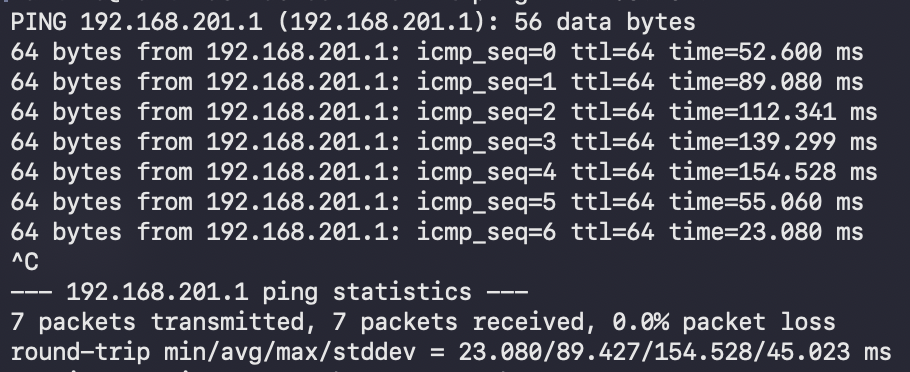
\includegraphics[width=0.8\textwidth]{1.png}
    \caption{Output atteso di un \texttt{ping} riuscito verso il robot.}
\end{figure}

Se la perdita di pacchetti è vicina allo 0\%, puoi continuare. Altrimenti, riprova il ping o verifica di essere correttamente connesso al WiFi del Dobot.

\item Connettiti via SSH:
\begin{lstlisting}[style=block,language=bash]
ssh root@192.168.201.1
\end{lstlisting}
Questo passaggio potrebbe richiedere una password, solitamente ``dobot''.

\item Esegui il backup delle impostazioni attuali:
\begin{lstlisting}[style=block,language=bash]
cp /dobot/userdata/project/settings/function/remoteControl.json /dobot/userdata/project/settings/function/remoteControl.json.bak
\end{lstlisting}

\item Imposta la modalità TCP:
\begin{lstlisting}[style=block,language=bash]
echo '{"mode":"tcp"}' > /dobot/userdata/project/settings/function/remoteControl.json
echo '{"mode":"tcp"}' > /dobot/userdata/user_project/settings/function/remoteControl.json
\end{lstlisting}

\item Attiva l'interruttore remoto:
\begin{lstlisting}[style=block,language=bash]
echo '{"value": true}' > /dobot/userdata/project/settings/function/remoteSwitch.json
echo '{"value": true}' > /dobot/userdata/user_project/settings/function/remoteSwitch.json
\end{lstlisting}

\item Riavvia:
\begin{lstlisting}[style=block,language=bash]
reboot
\end{lstlisting}

\item Poi spegni il Dobot tenendo premuto il pulsante on/off per 4 secondi, attendi 30s e riaccendilo premendo una volta il pulsante on/off.

\end{enumerate}

\subsubsection*{Disattivare la modalità TCP}

\begin{enumerate}[leftmargin=1.2cm]

\item Accendi il Dobot, attendi che si avvii completamente e si connetta al suo WiFi. Apri il terminale.

I seguenti blocchi di codice includono l'IP di esempio \code{192.168.201.1}, che dovrai sostituire con l'IP del tuo Dobot.

Sia per utenti Mac che Windows:

\item Verifica la connessione del robot:
\begin{lstlisting}[style=block,language=bash]
ping 192.168.201.1
\end{lstlisting}

Su Mac, dopo un po' dovrai interromperlo con Control+C.

Se eseguito correttamente, otterrai qualcosa del genere:

\begin{figure}[H]
    \centering
    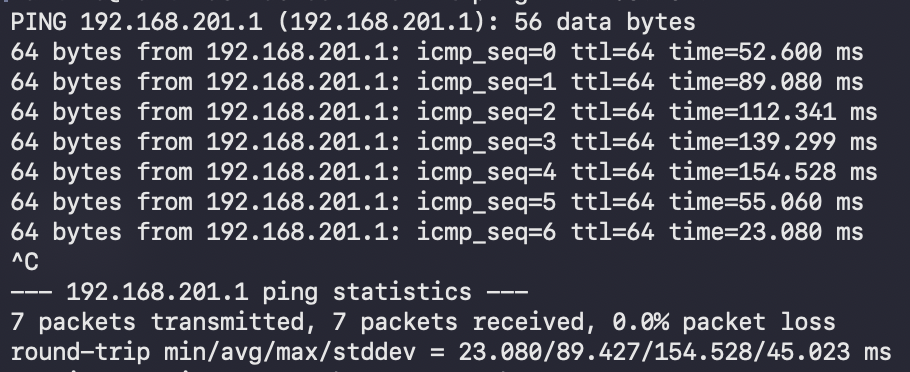
\includegraphics[width=0.8\textwidth]{2.png}
    \caption{Output atteso di un \texttt{ping} riuscito verso il robot.}
\end{figure}

Se la perdita di pacchetti è vicina allo 0\%, puoi continuare. Altrimenti, riprova il ping o verifica di essere correttamente connesso al WiFi del Dobot.

\item Connettiti via SSH:
\begin{lstlisting}[style=block,language=bash]
ssh root@192.168.201.1
\end{lstlisting}
Questo passaggio potrebbe richiedere una password, solitamente ``dobot''.

\item Esegui il backup delle impostazioni attuali:
\begin{lstlisting}[style=block,language=bash]
cp /dobot/userdata/project/settings/function/remoteControl.json /dobot/userdata/project/settings/function/remoteControl.json.bak
\end{lstlisting}

\item Imposta la modalità TP:
\begin{lstlisting}[style=block,language=bash]
echo '{"mode":"tp"}' > /dobot/userdata/project/settings/function/remoteControl.json
echo '{"mode":"tp"}' > /dobot/userdata/user_project/settings/function/remoteControl.json
\end{lstlisting}

\item Disattiva l'interruttore remoto:
\begin{lstlisting}[style=block,language=bash]
echo '{"value": false}' > /dobot/userdata/project/settings/function/remoteSwitch.json
echo '{"value": false}' > /dobot/userdata/user_project/settings/function/remoteSwitch.json
\end{lstlisting}

\item Riavvia:
\begin{lstlisting}[style=block,language=bash]
reboot
\end{lstlisting}

\item Poi spegni il Dobot tenendo premuto il pulsante on/off per 4 secondi, attendi 30s e riaccendilo premendo una volta il pulsante on/off.

\end{enumerate}

% ============================================================
\section{Come usare DobotStudio Pro}
\label{sec:dobotstudio-guide}
% ============================================================

DobotStudio Pro è il software originale per controllare e programmare qualsiasi braccio robotico Dobot.

Di seguito una breve spiegazione delle principali funzionalità del software, ma ti consiglio di consultare il file ``DobotStudio Pro User Guide (CR\&Nova) V2.8.0'', scaricabile su \url{https://www.Dobot-robots.com/service/download-center}, oppure di visitare il sito \url{https://docs.trossenrobotics.com/Dobot_cr_cobots_docs/Dobotstudiopro/programming.html}, dove viene trattato in modo più approfondito.

\begin{itemize}[leftmargin=1.2cm]

\item Questa è la pagina con cui si apre il software. Con ``Connect'' potrai selezionare il tuo Dobot tramite il suo IP e connetterti. Assicurati di essere connesso al WiFi del Dobot.

\begin{figure}[H]
    \centering
    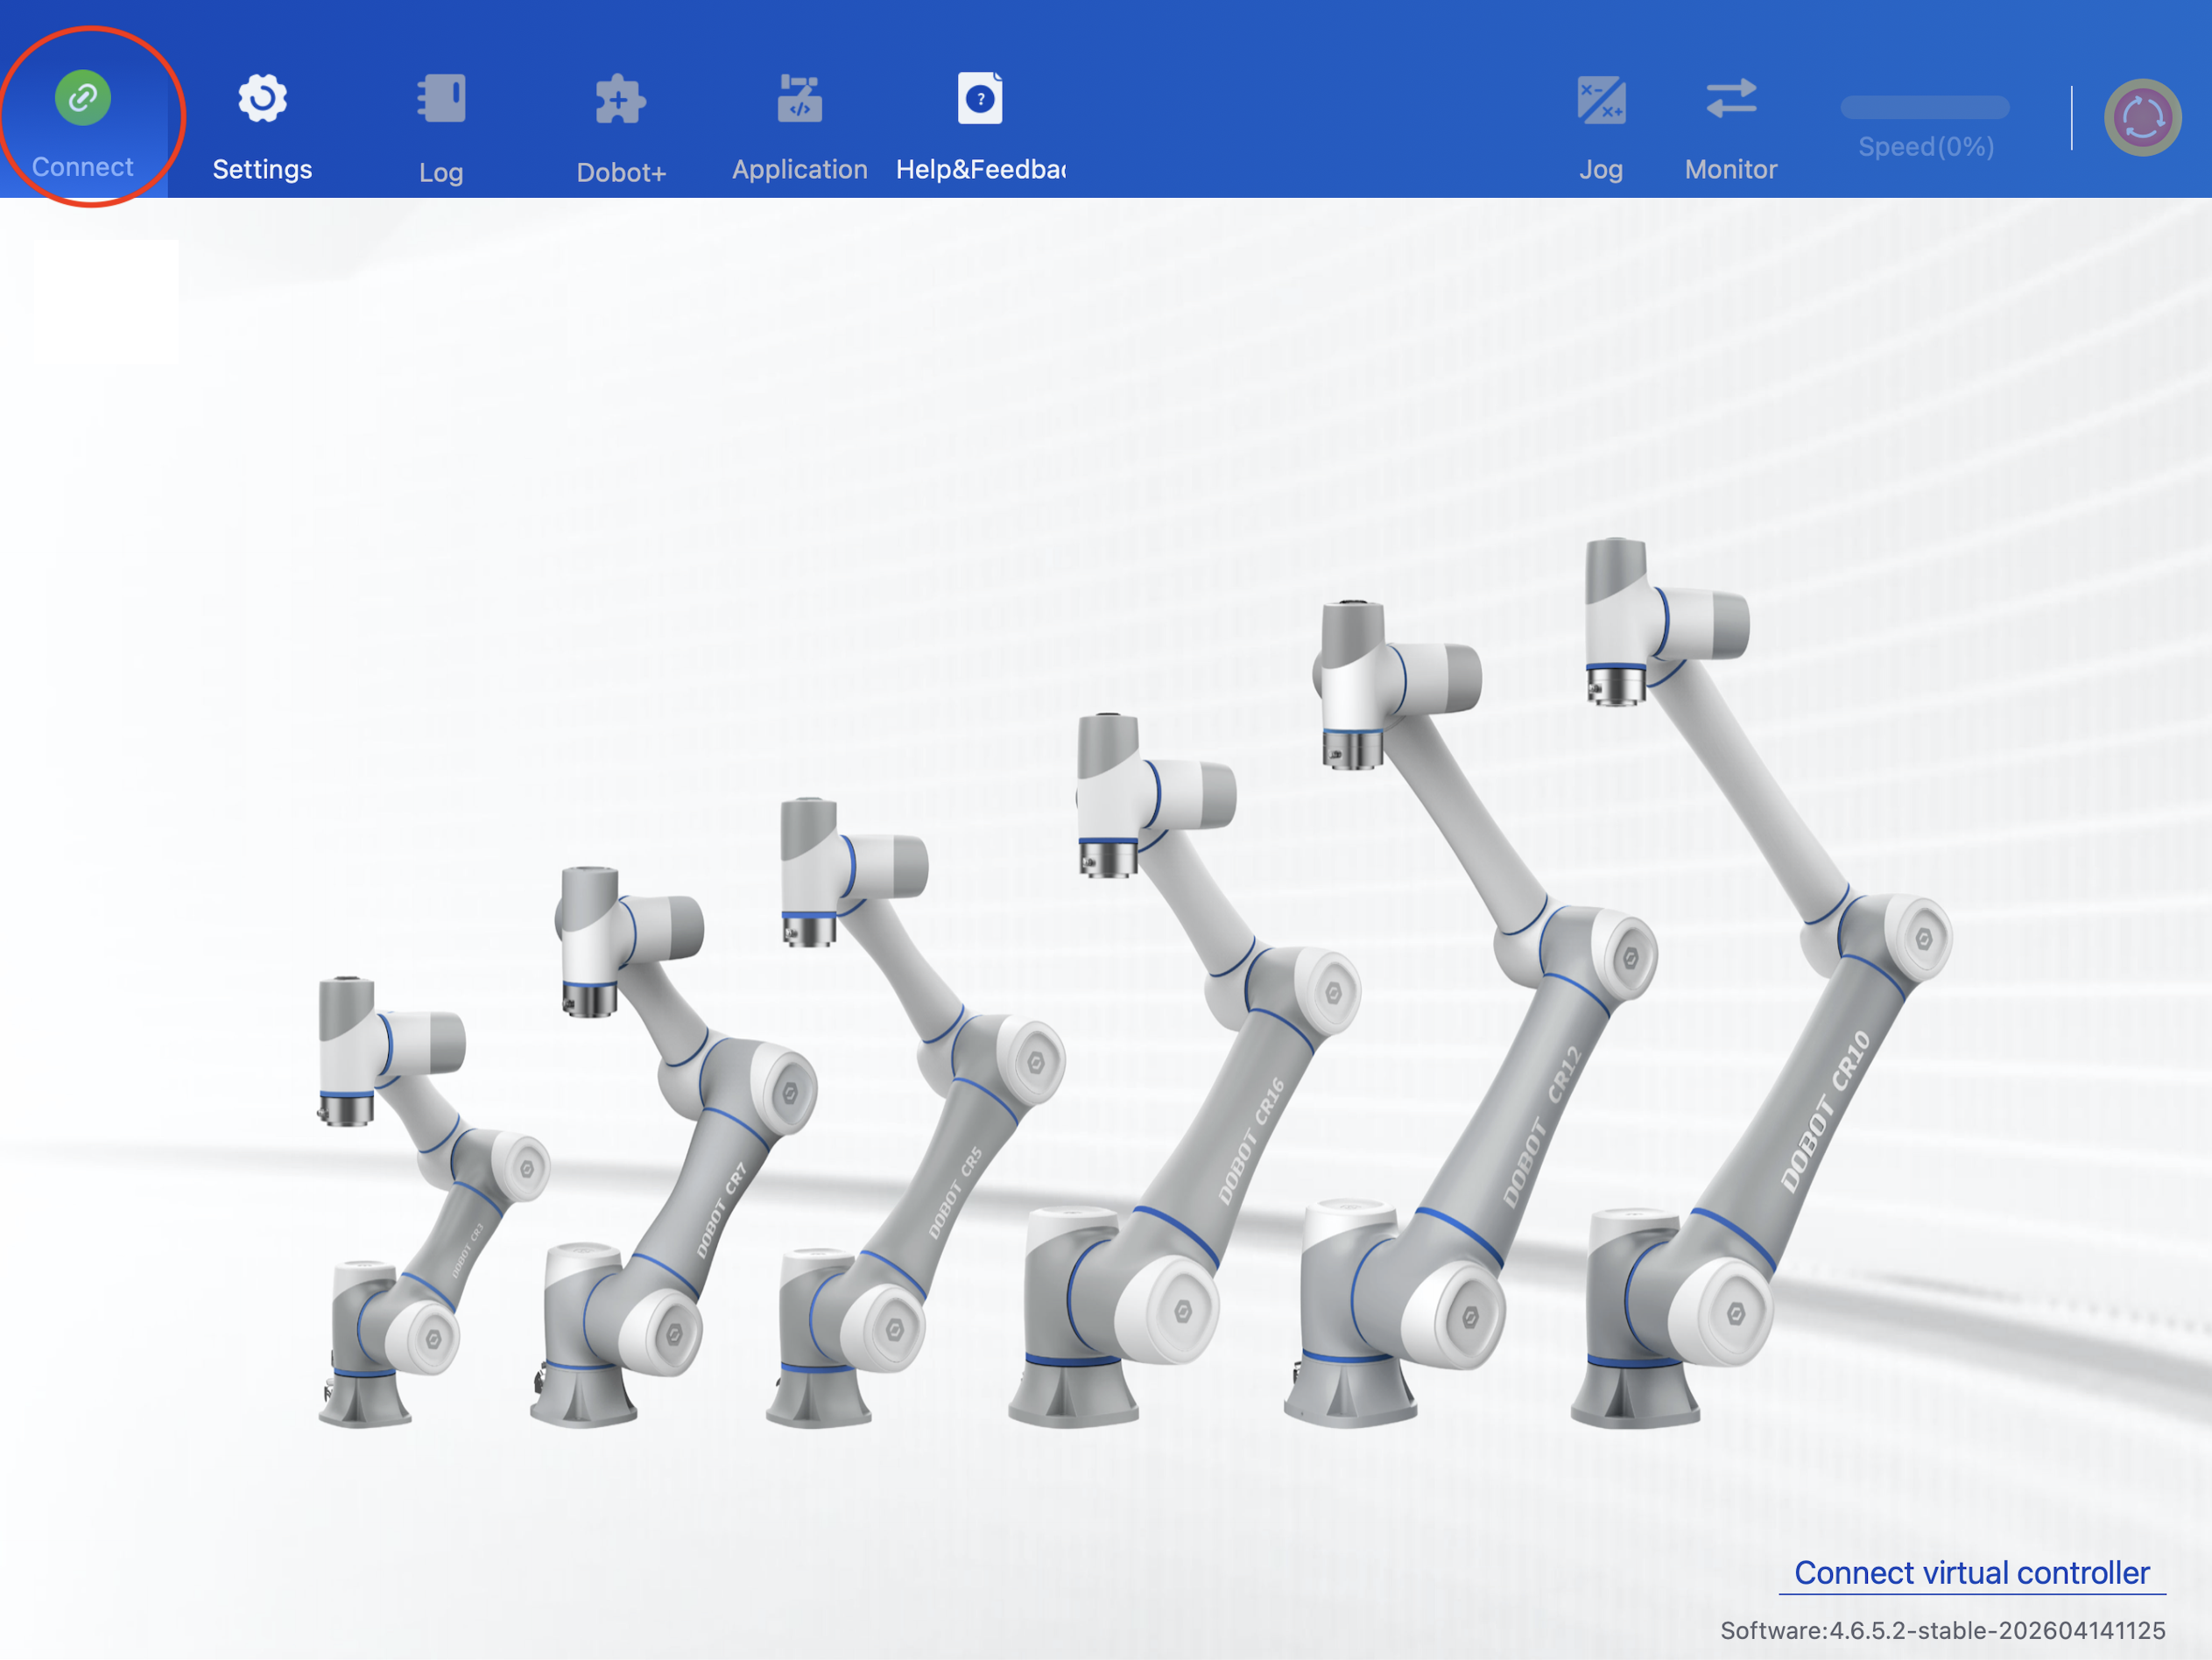
\includegraphics[width=0.9\textwidth]{3.png}
\end{figure}

\item Premendo ``Enable'' abiliti il Dobot a essere controllato. Nota che sul lato destro dello schermo puoi vedere la posizione del Dobot in ogni momento e, se SafeSkin è attivo, verificare se alcune parti rilevano un oggetto vicino.

Il colore della piccola icona del Dobot nell'angolo in alto a sinistra indica il suo stato: blu significa disabilitato, verde significa abilitato e funzionante correttamente, giallo indica un errore non pericoloso (come una collisione rilevata da SafeSkin), e rosso indica un errore pericoloso.

\begin{figure}[H]
    \centering
    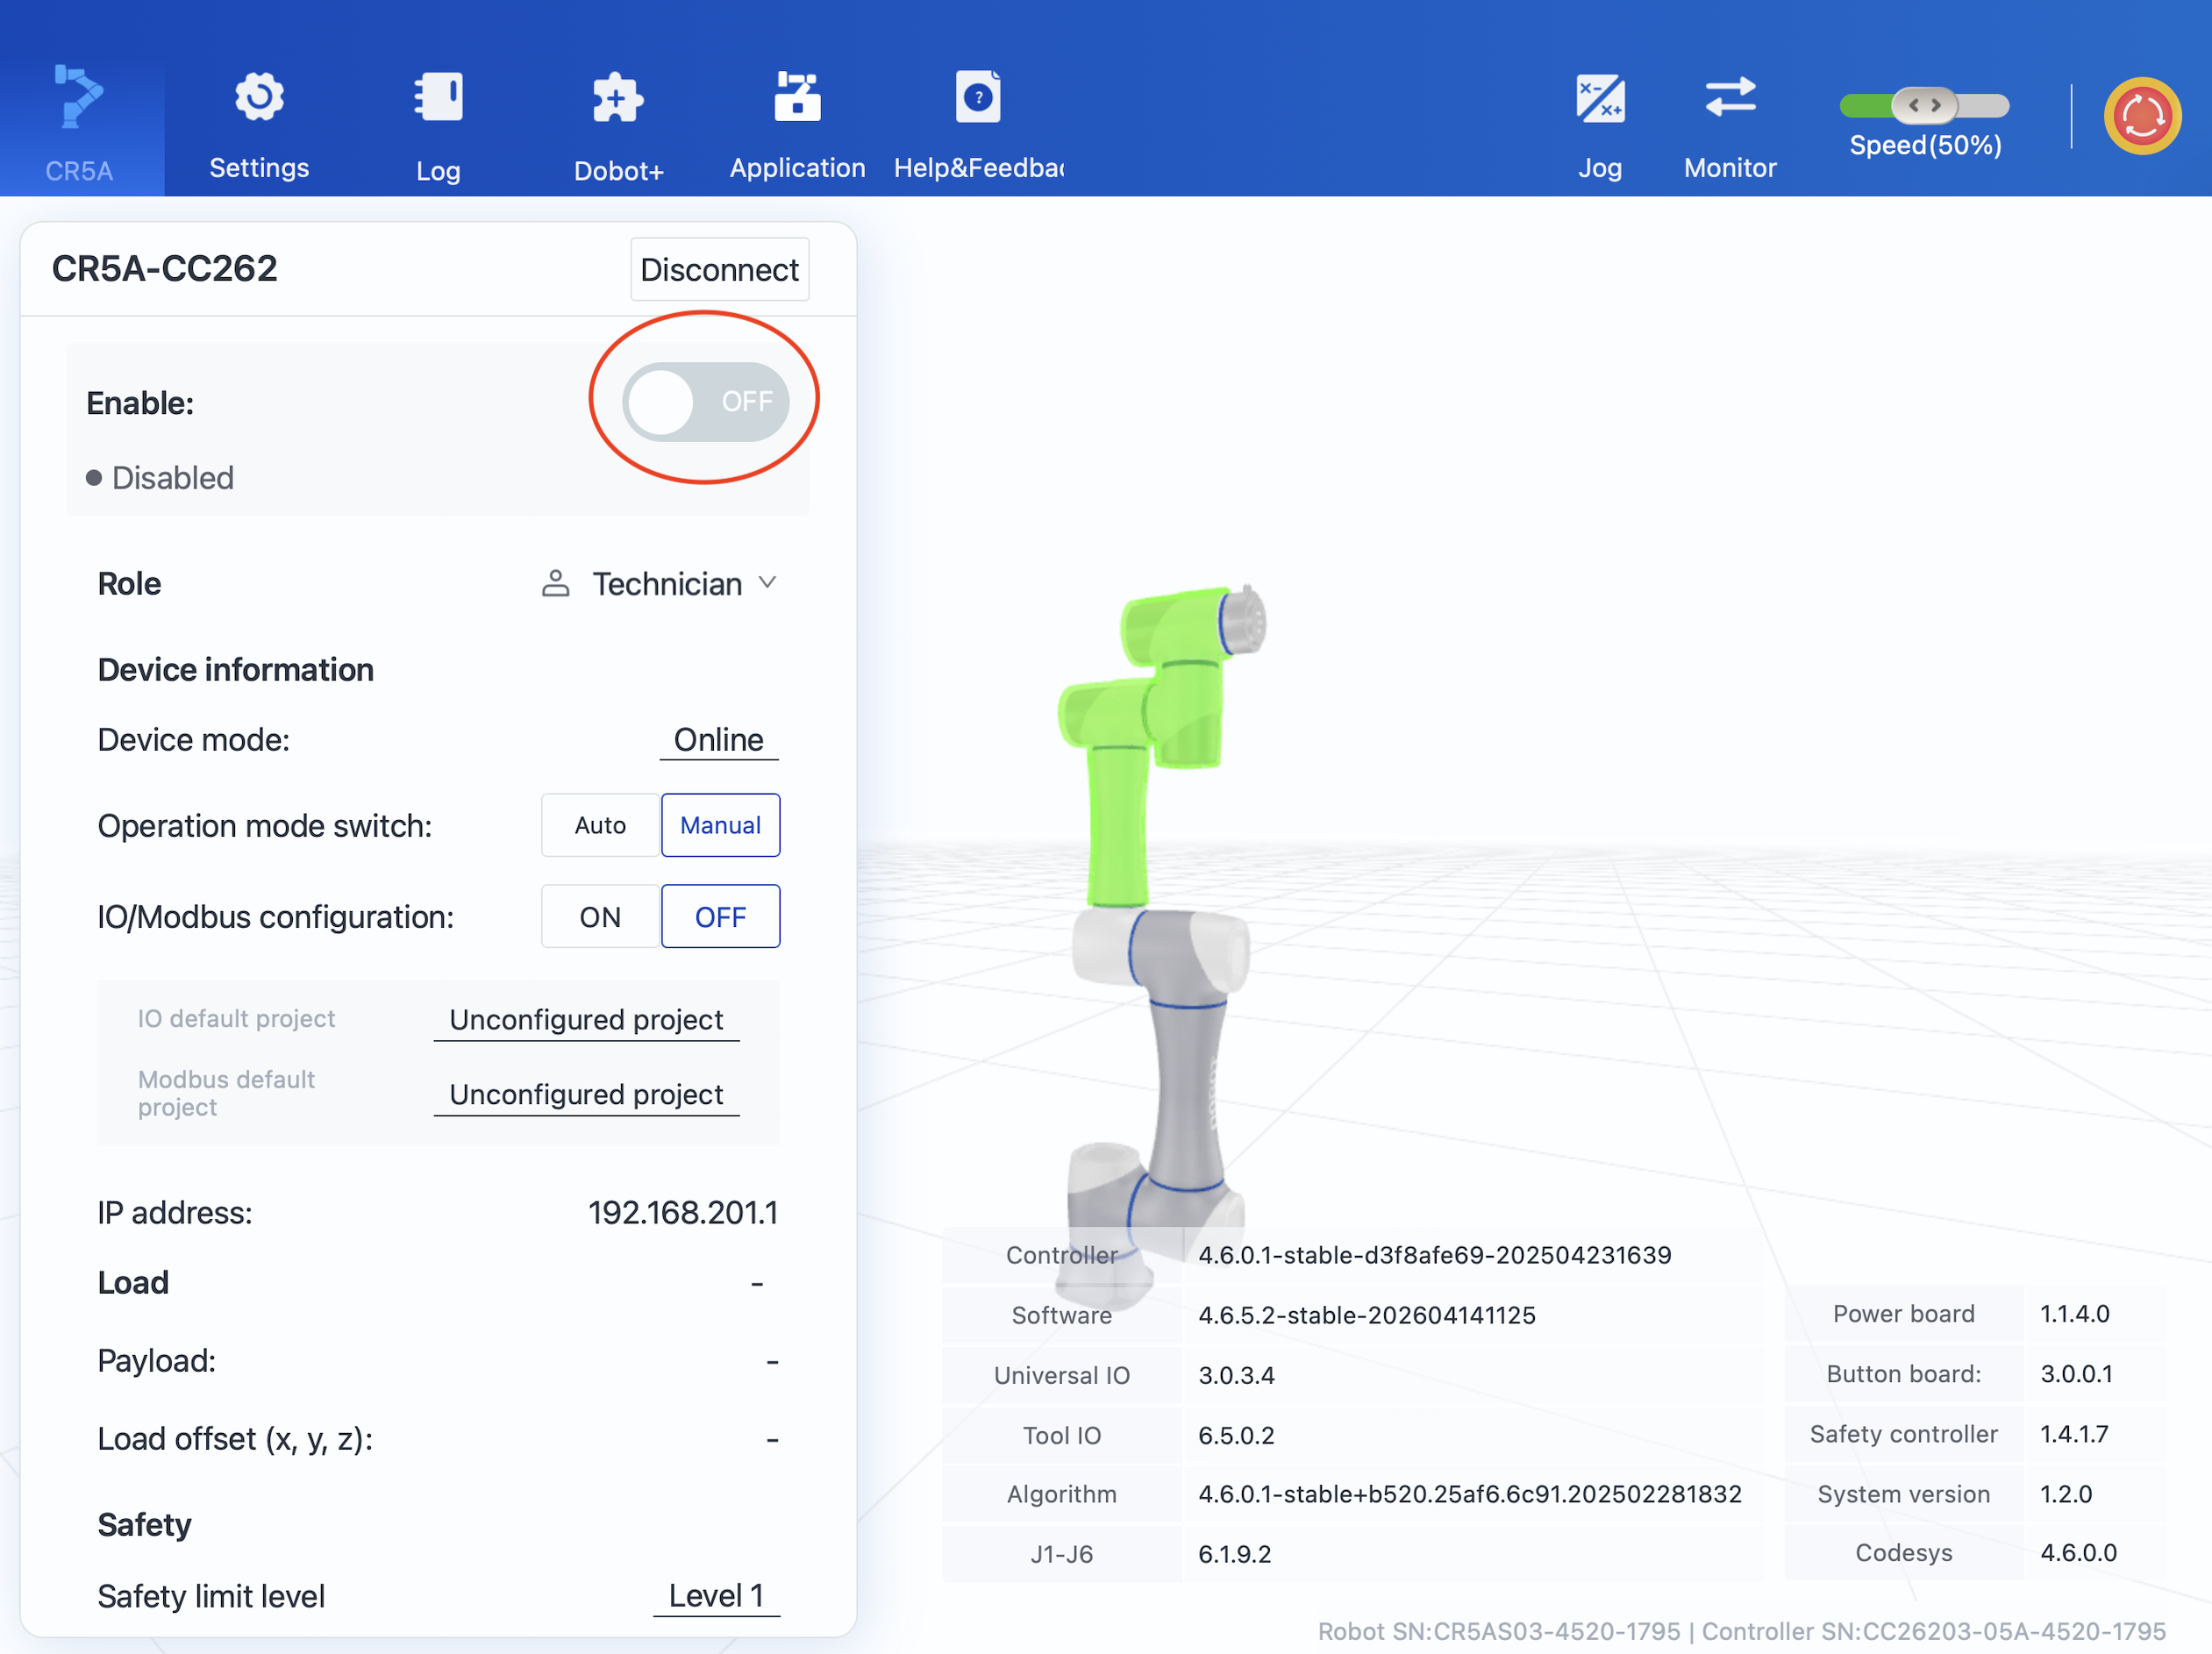
\includegraphics[width=0.9\textwidth]{4.png}
\end{figure}

\item Una volta premuto Enable, il Dobot eseguirà un esame del carico (Load examination). Se i numeri sono corretti, conferma Enable.

\begin{figure}[H]
    \centering
    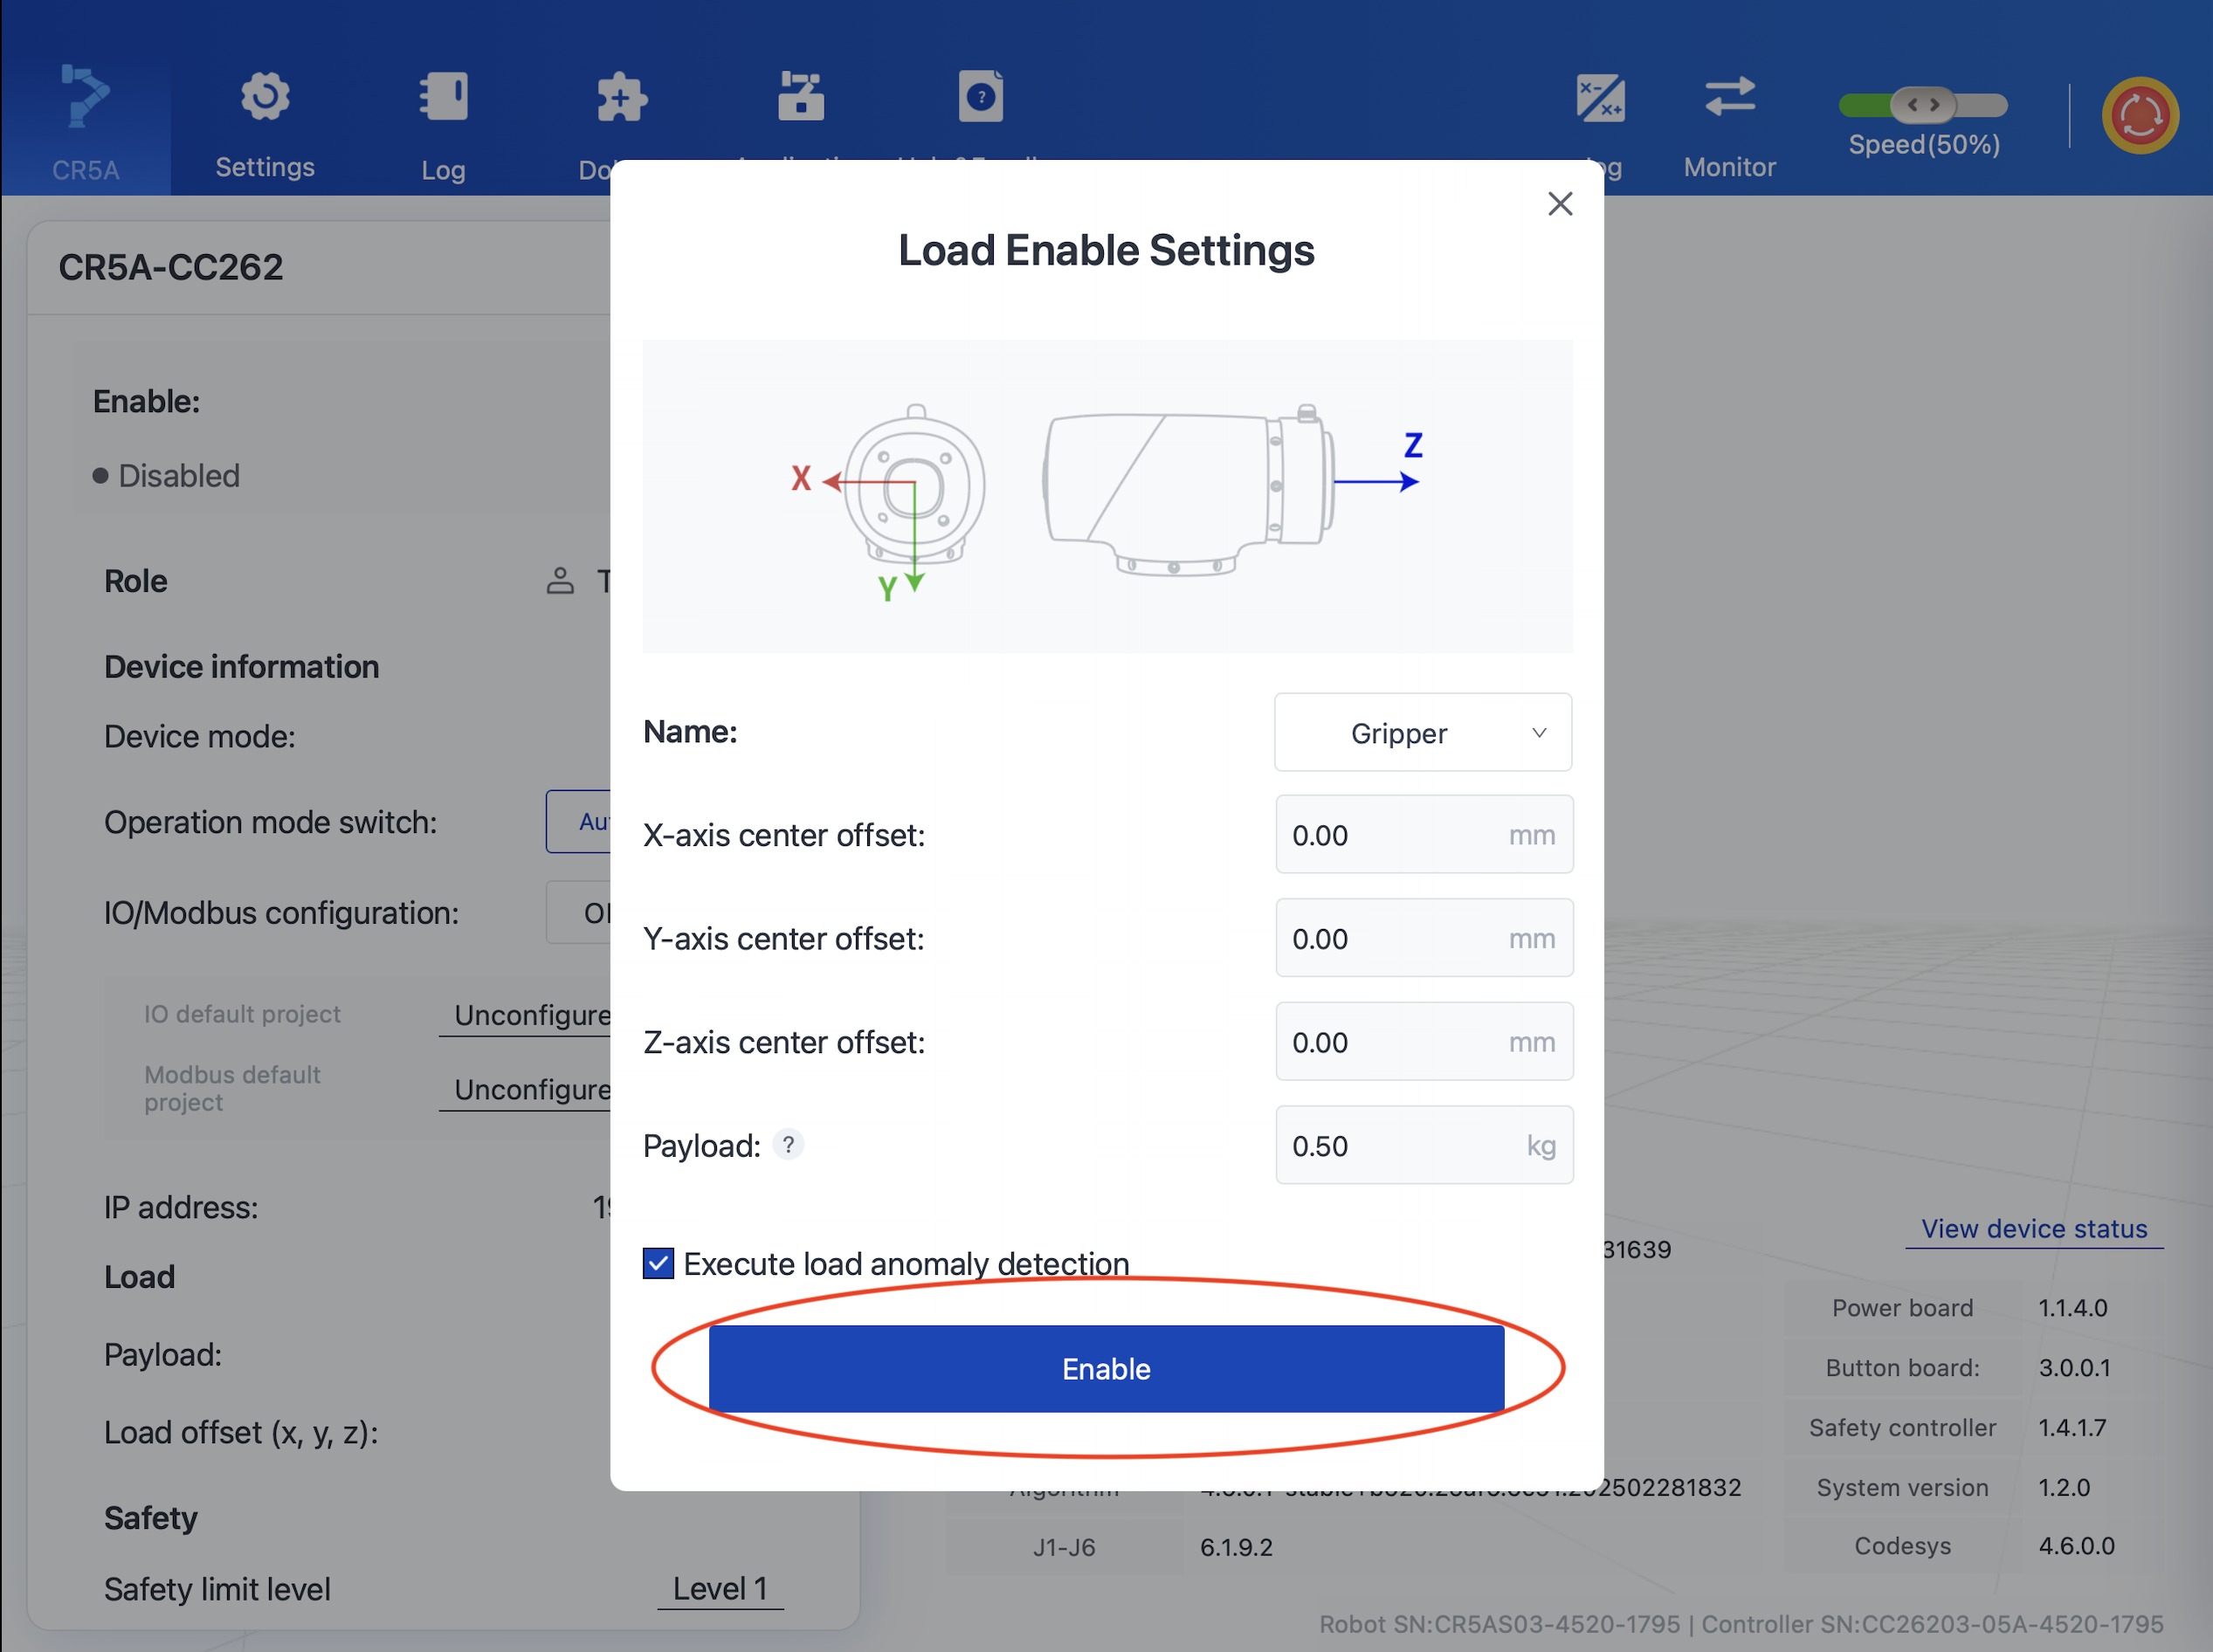
\includegraphics[width=0.9\textwidth]{5.png}
\end{figure}

\item Selezionando ``Jog'' puoi muovere il Dobot un giunto alla volta. Questa opzione include anche ``Target Pose'', con cui potrai spostare gradualmente il Dobot verso alcune posizioni predefinite come Safe Home e Pack Pose.

\begin{figure}[H]
    \centering
    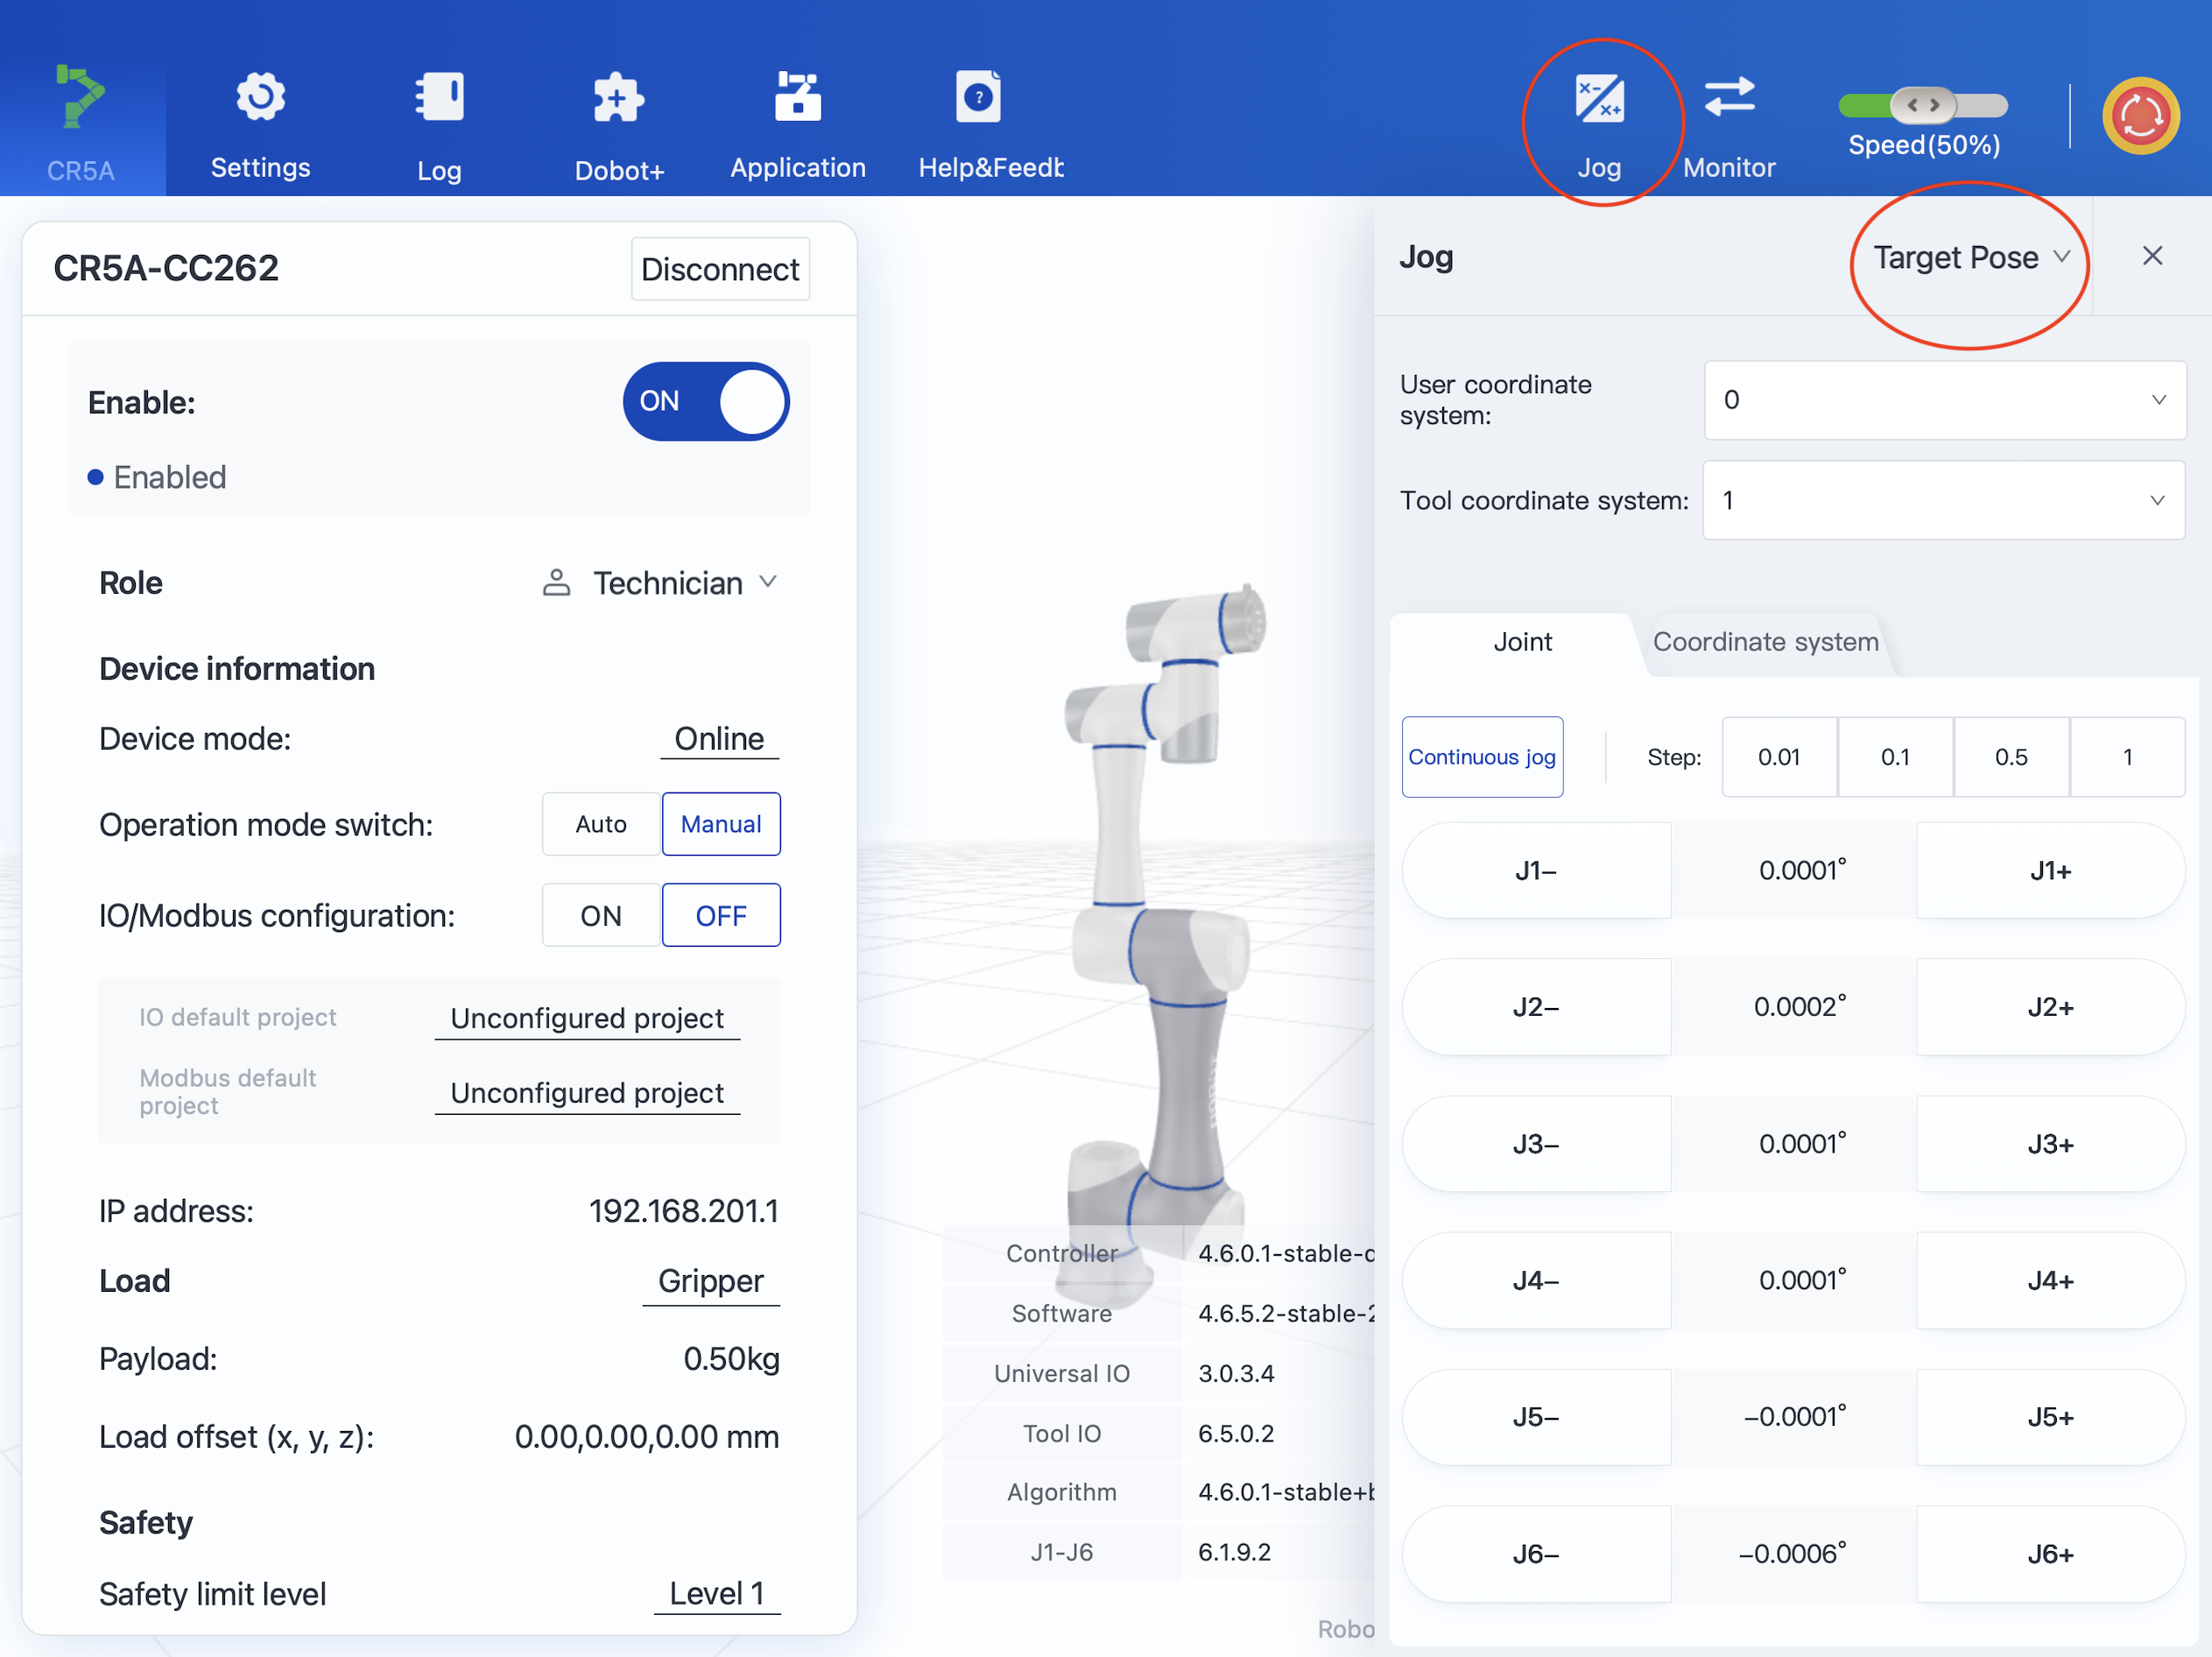
\includegraphics[width=0.9\textwidth]{6.png}
\end{figure}

\begin{figure}[H]
    \centering
    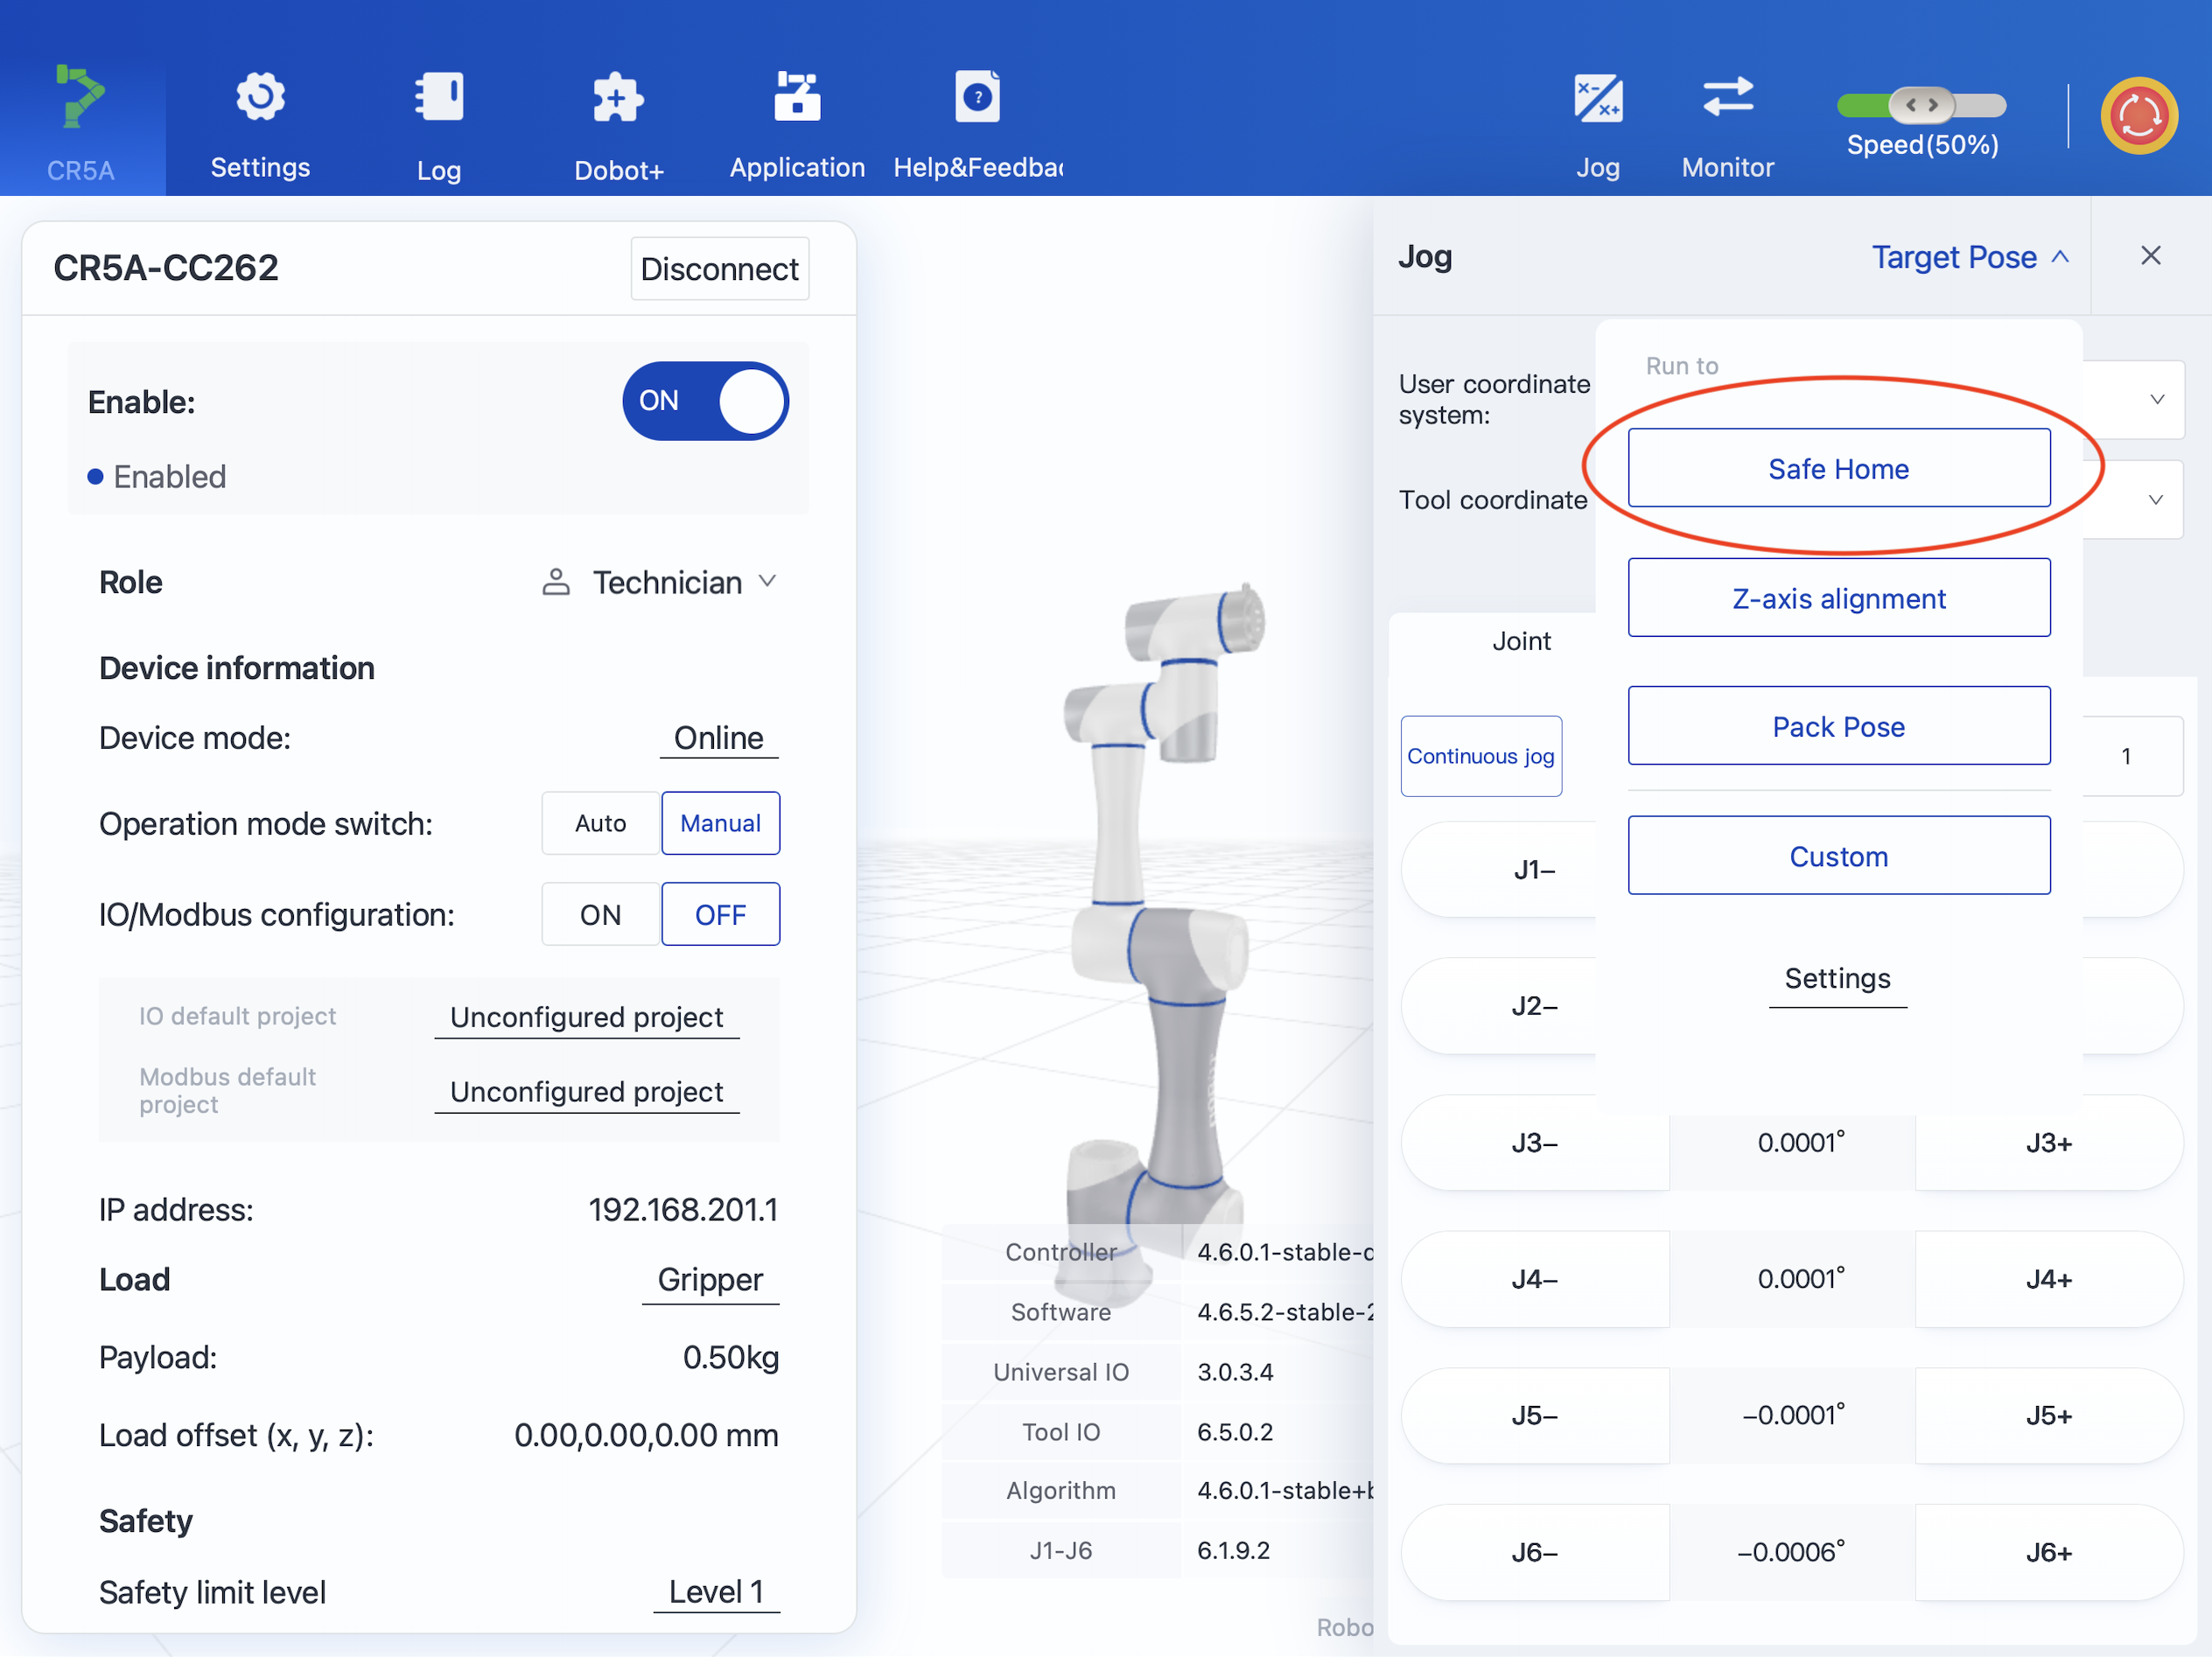
\includegraphics[width=0.9\textwidth]{7.png}
\end{figure}

\item Selezionando ``Monitor'' potrai accedere a ulteriori funzioni relative agli Input/Output.

\begin{figure}[H]
    \centering
    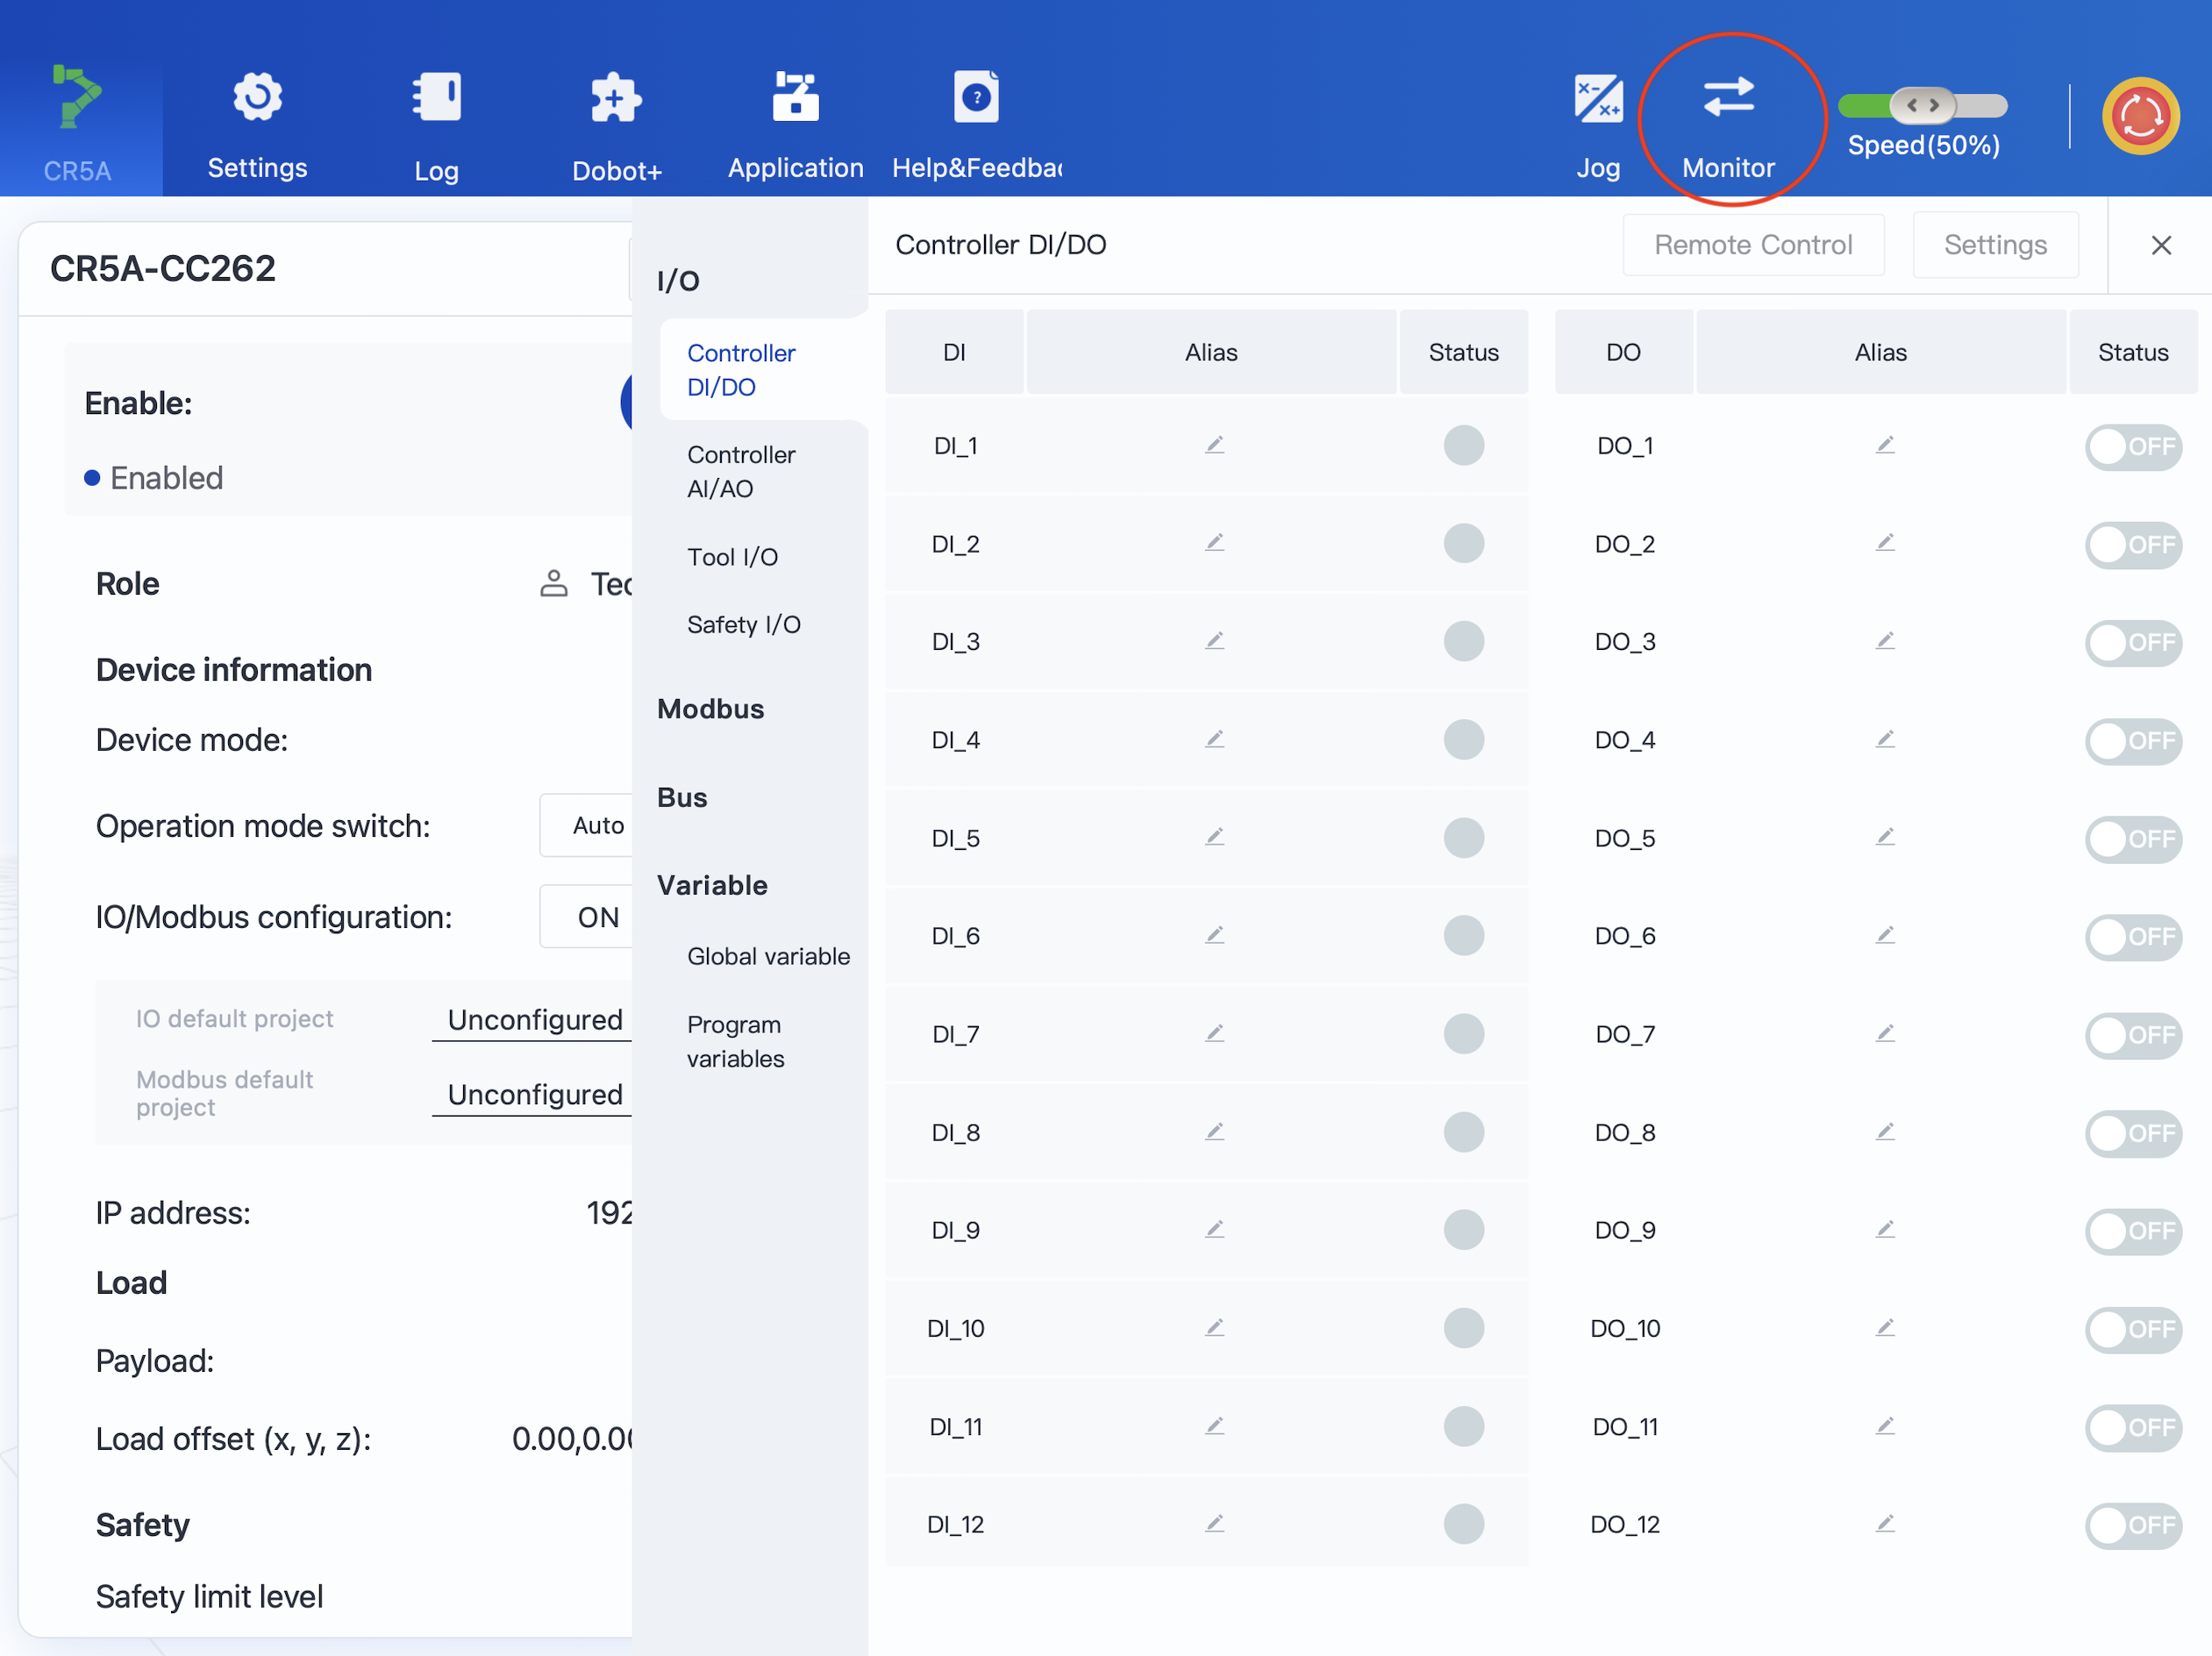
\includegraphics[width=0.9\textwidth]{8.png}
\end{figure}

\item Questo è il pannello Settings, che permette di configurare il Dobot. Un'impostazione importante da notare è che entrando in ``Communications'' potrai visualizzare e modificare l'indirizzo IP del Dobot.

\begin{figure}[H]
    \centering
    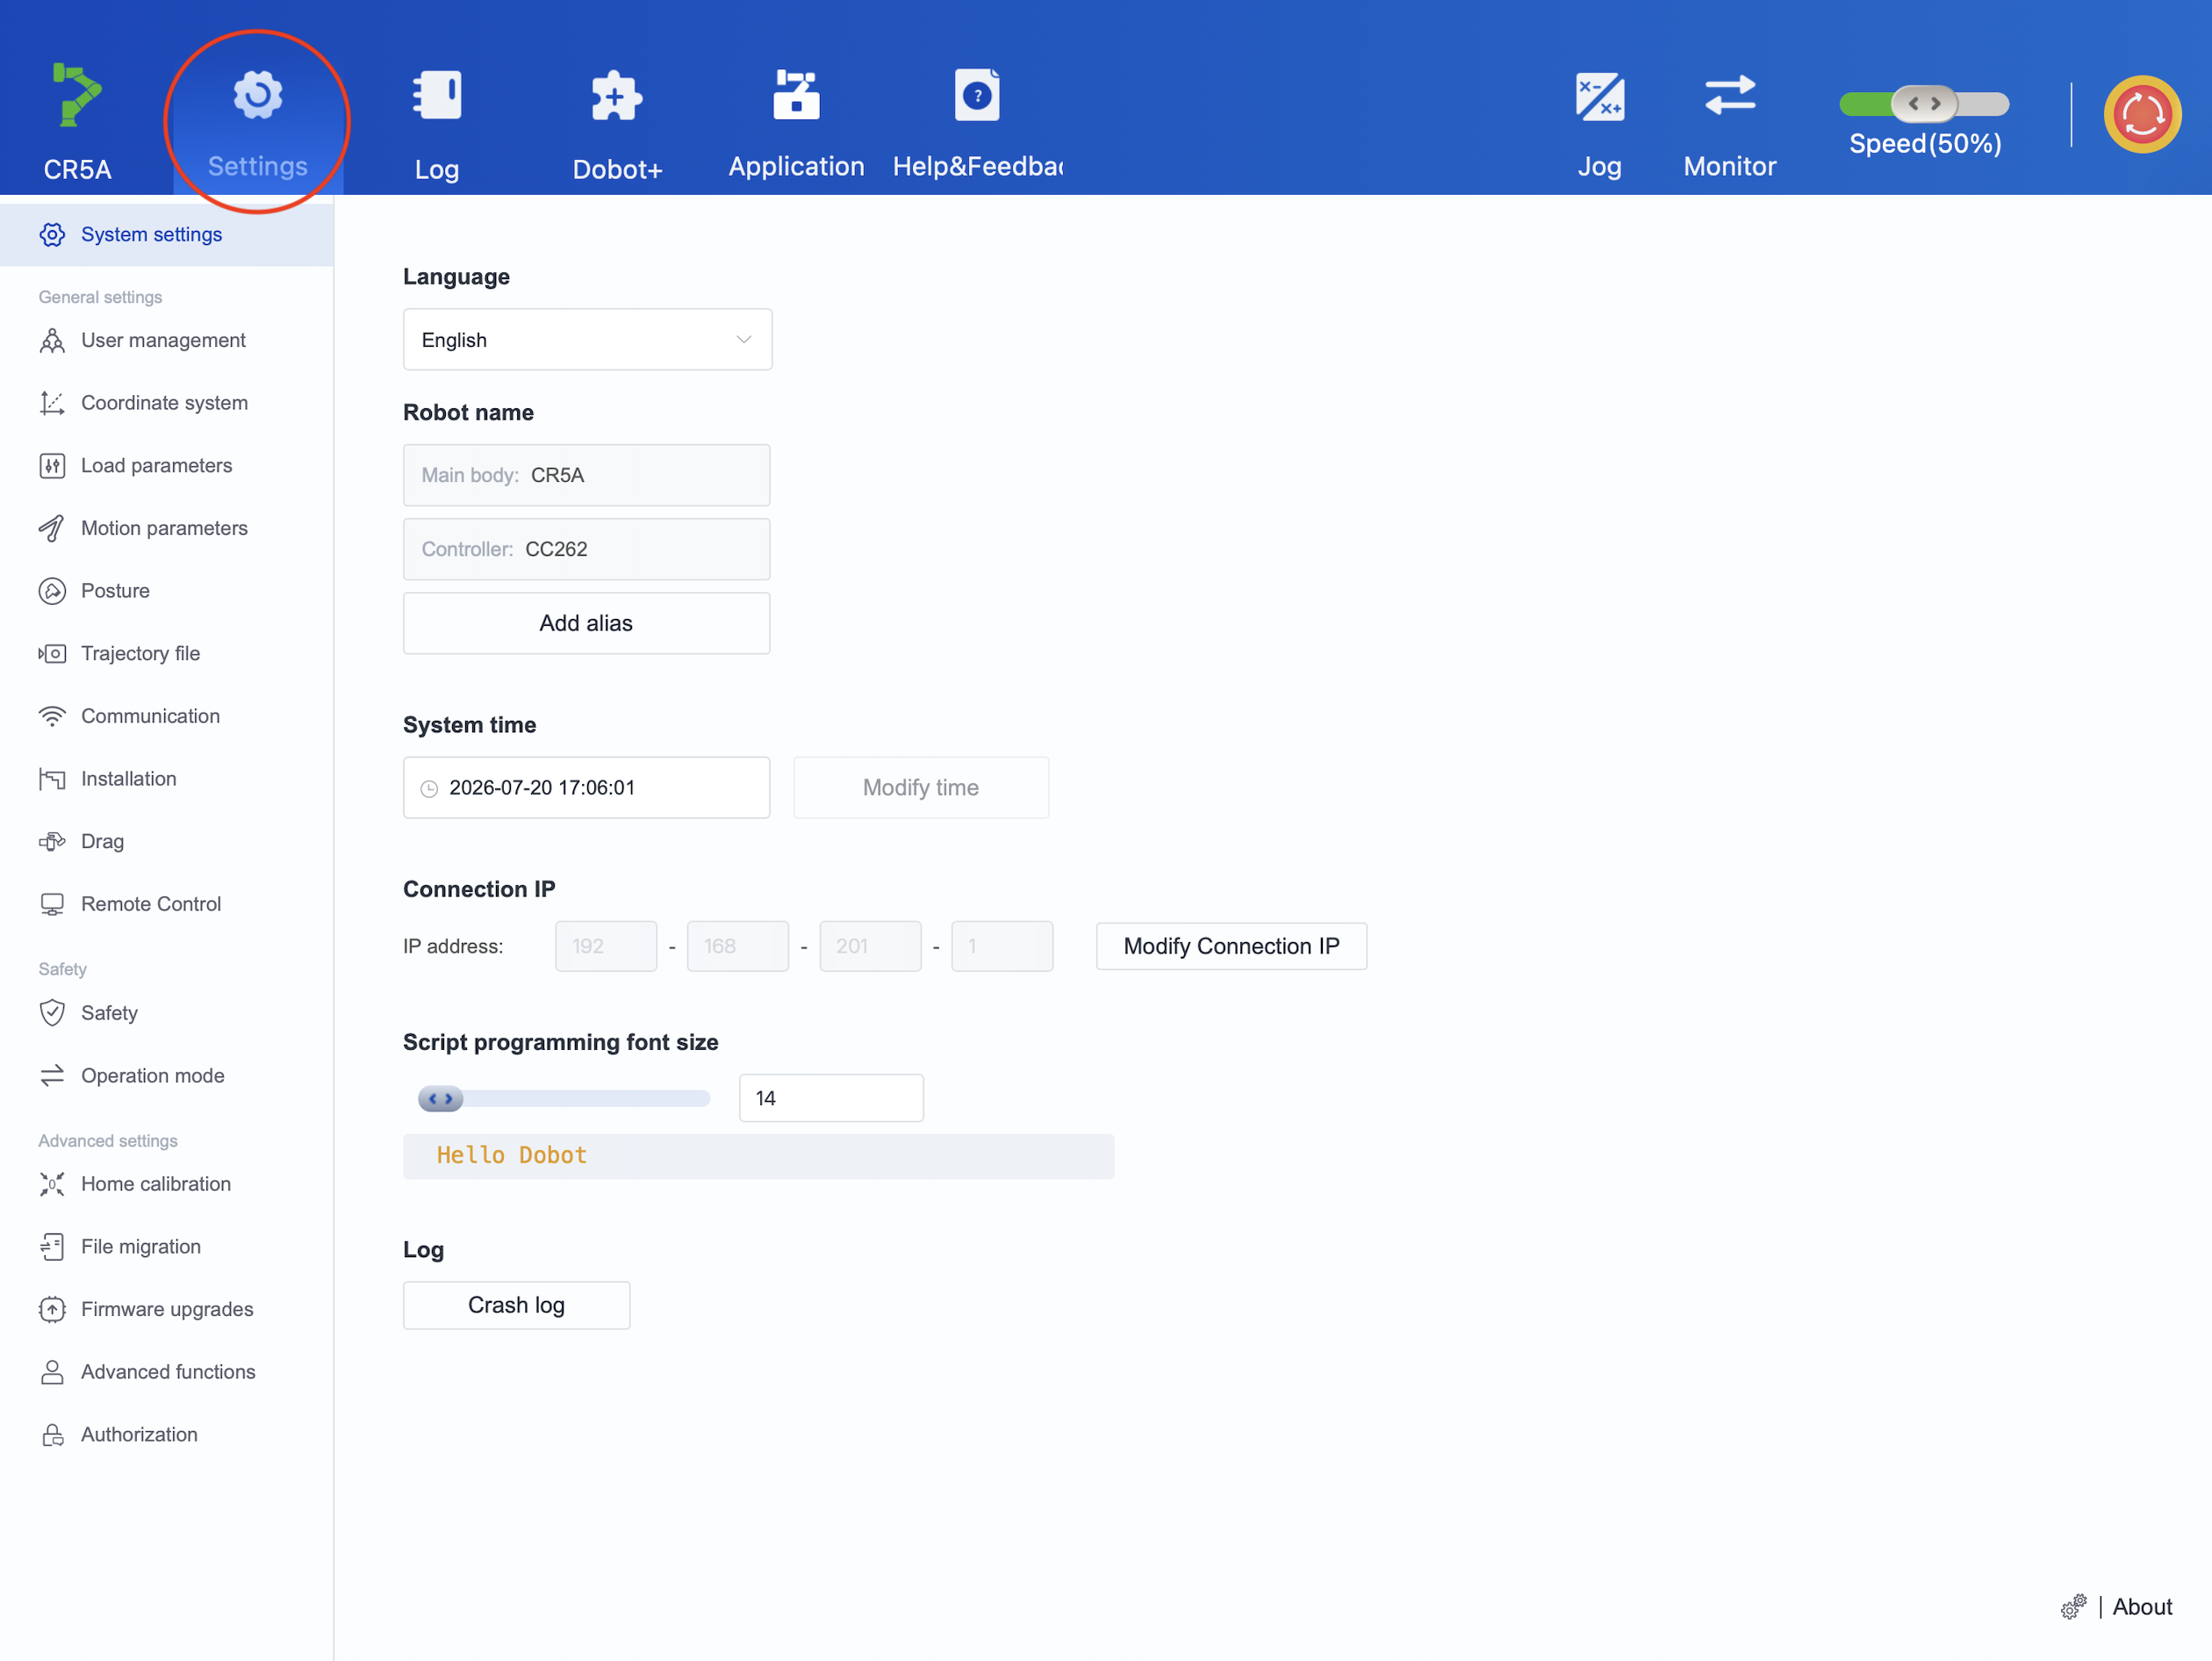
\includegraphics[width=0.9\textwidth]{9.png}
\end{figure}

\begin{figure}[H]
    \centering
    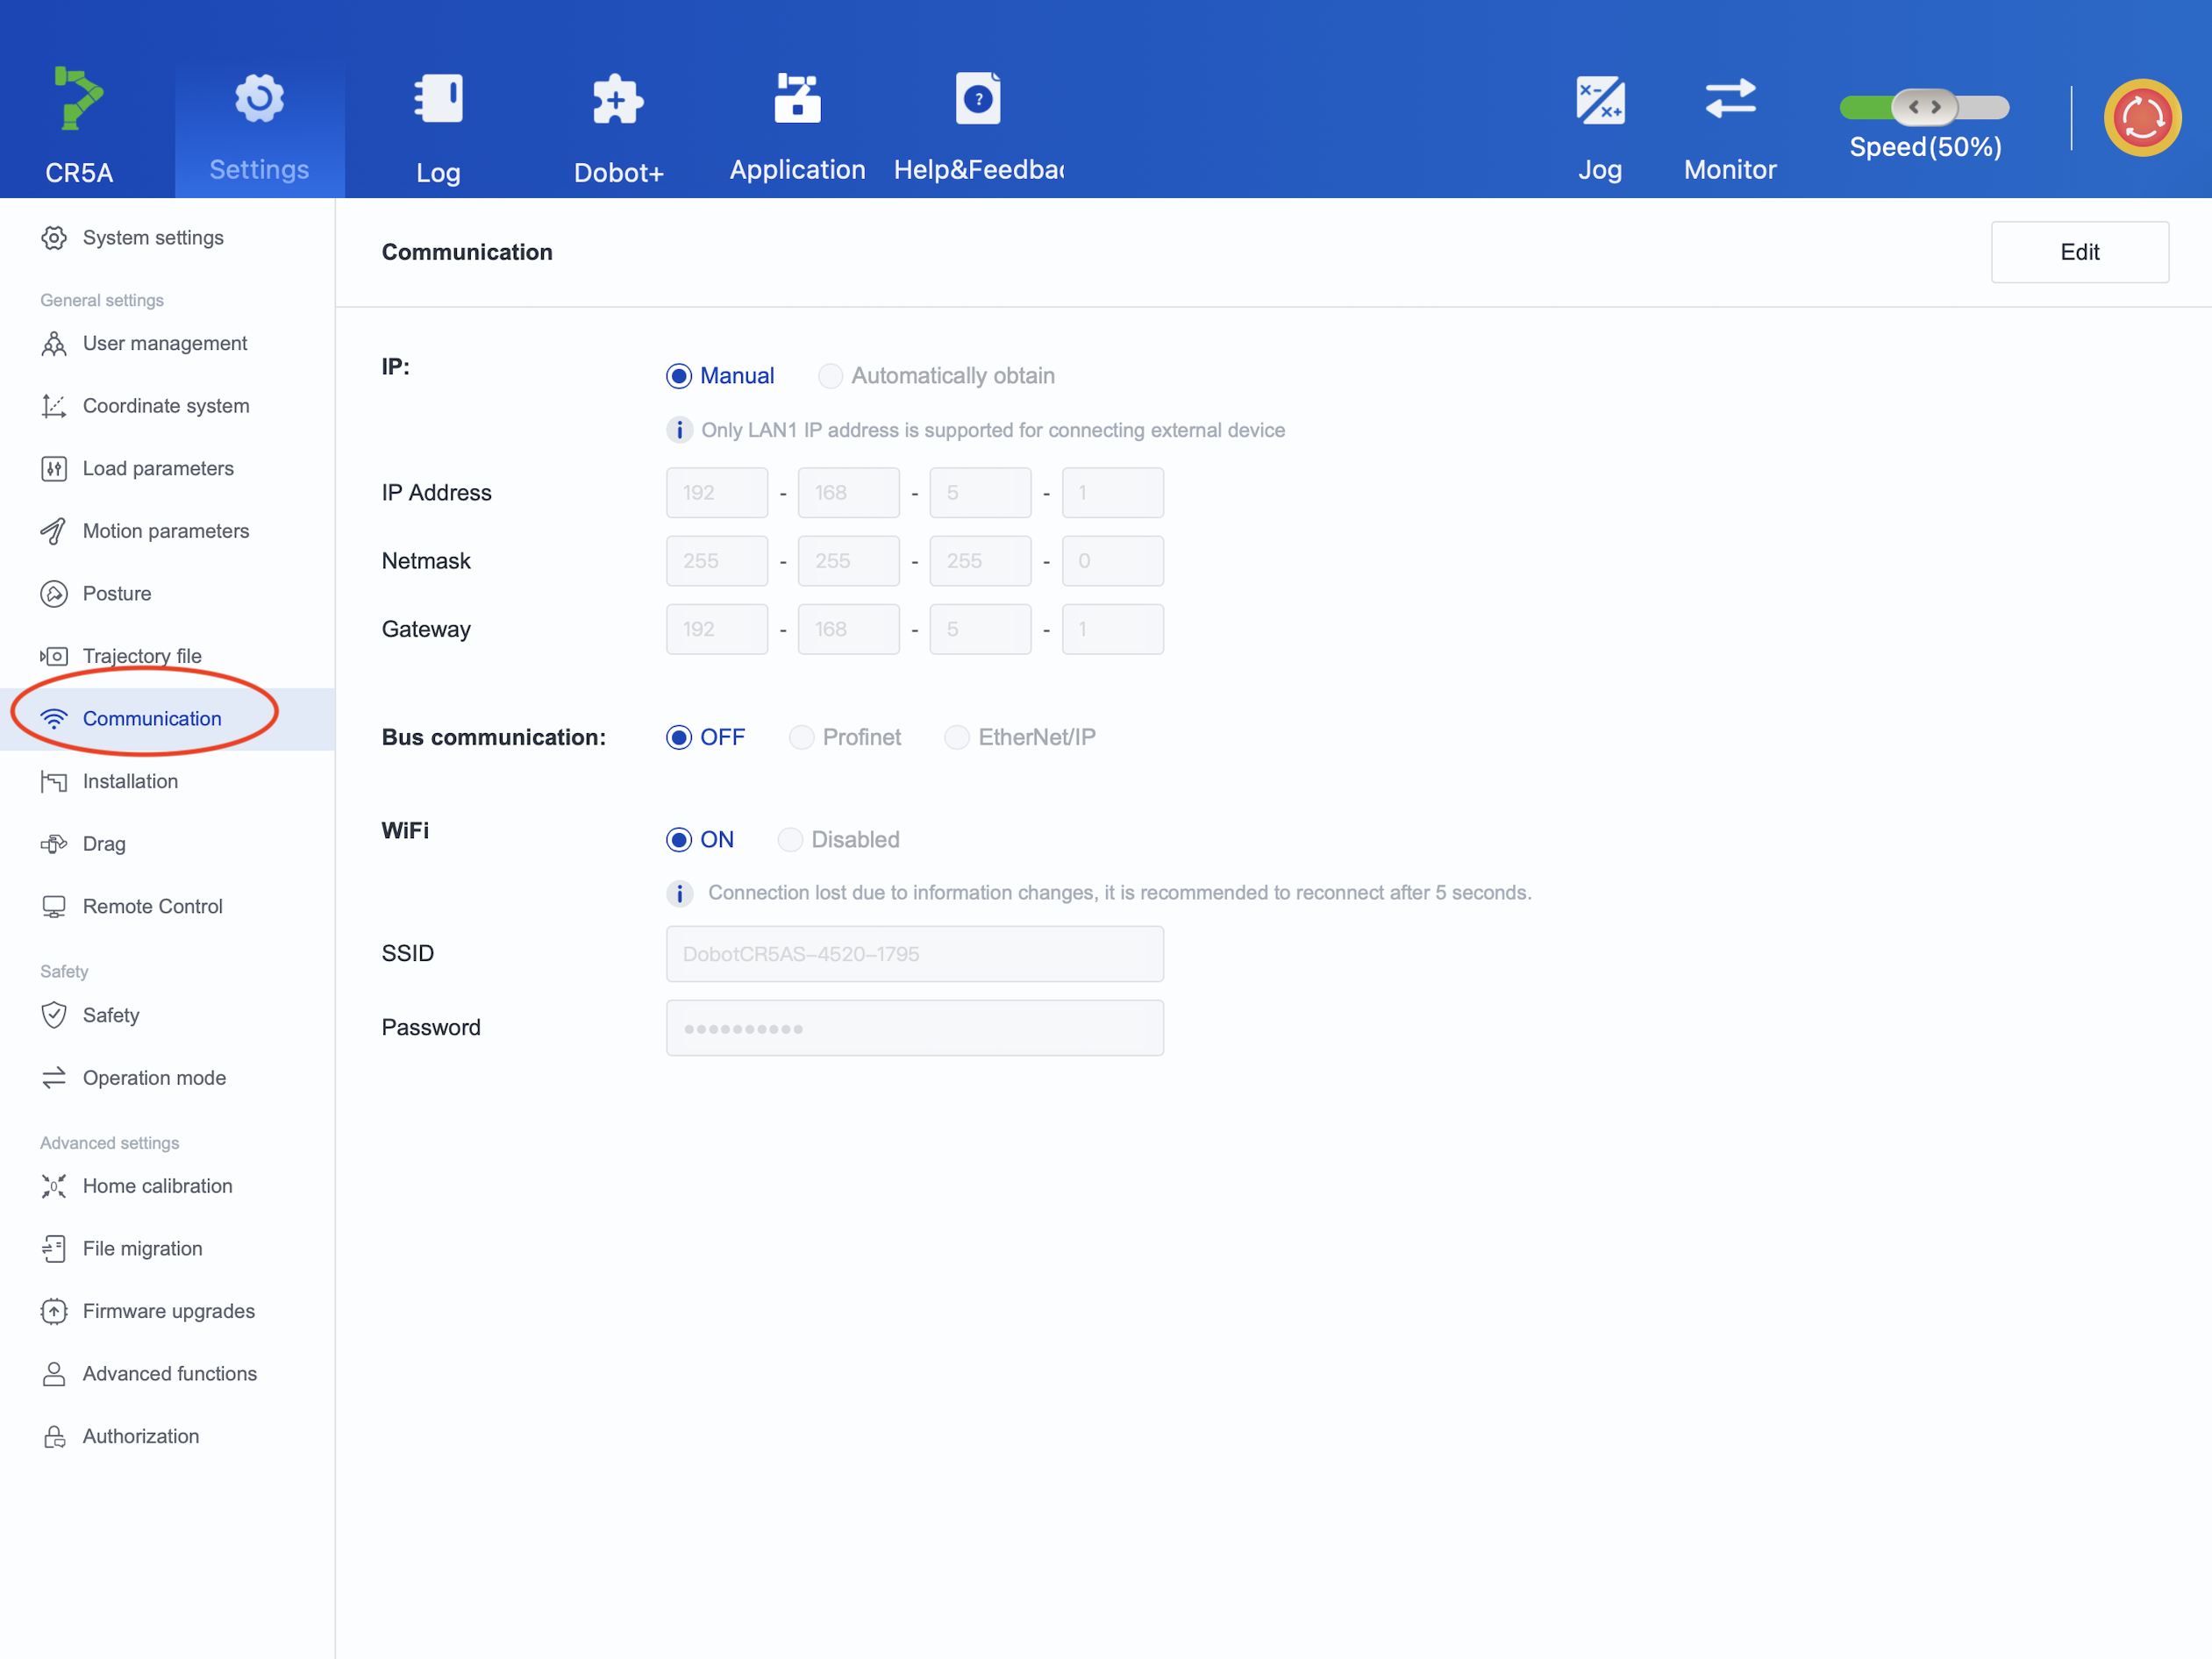
\includegraphics[width=0.9\textwidth]{10.png}
\end{figure}

\item Premendo ``Dobot+'' potrai esplorare le estensioni; alcune importanti sono le estensioni Gripper e SafeSkin.

\begin{figure}[H]
    \centering
    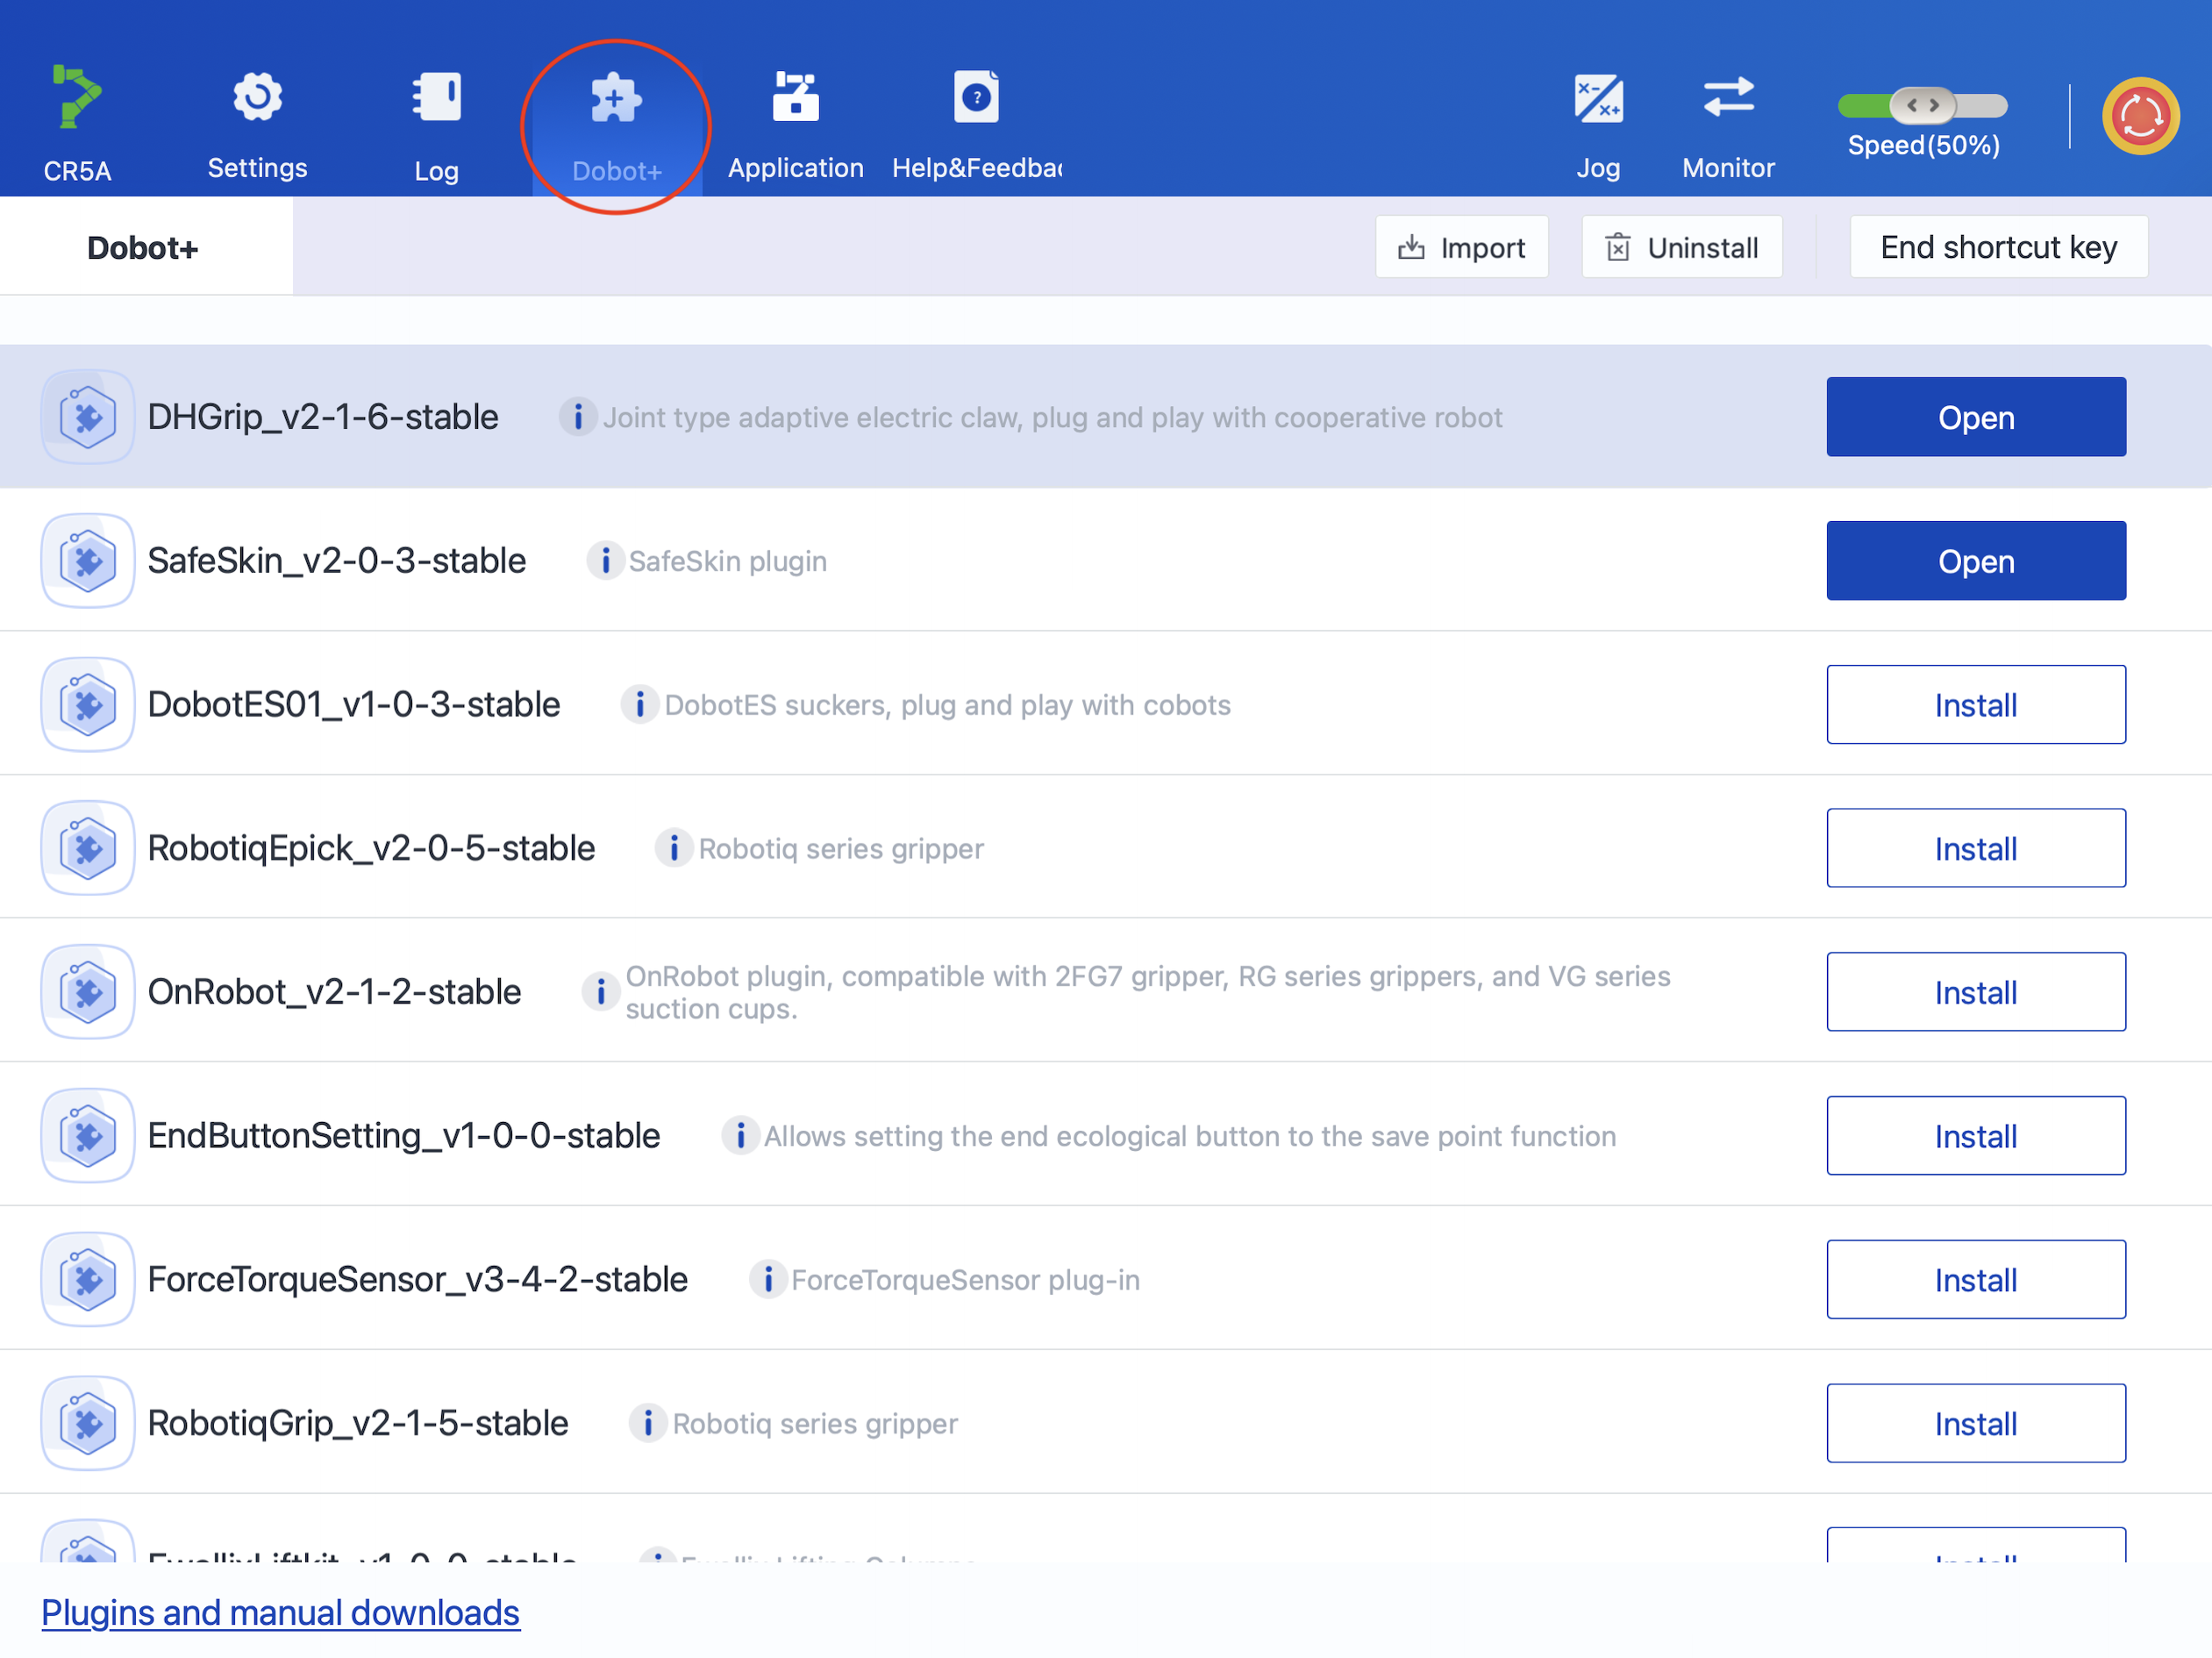
\includegraphics[width=0.9\textwidth]{11.png}
\end{figure}

\begin{figure}[H]
    \centering
    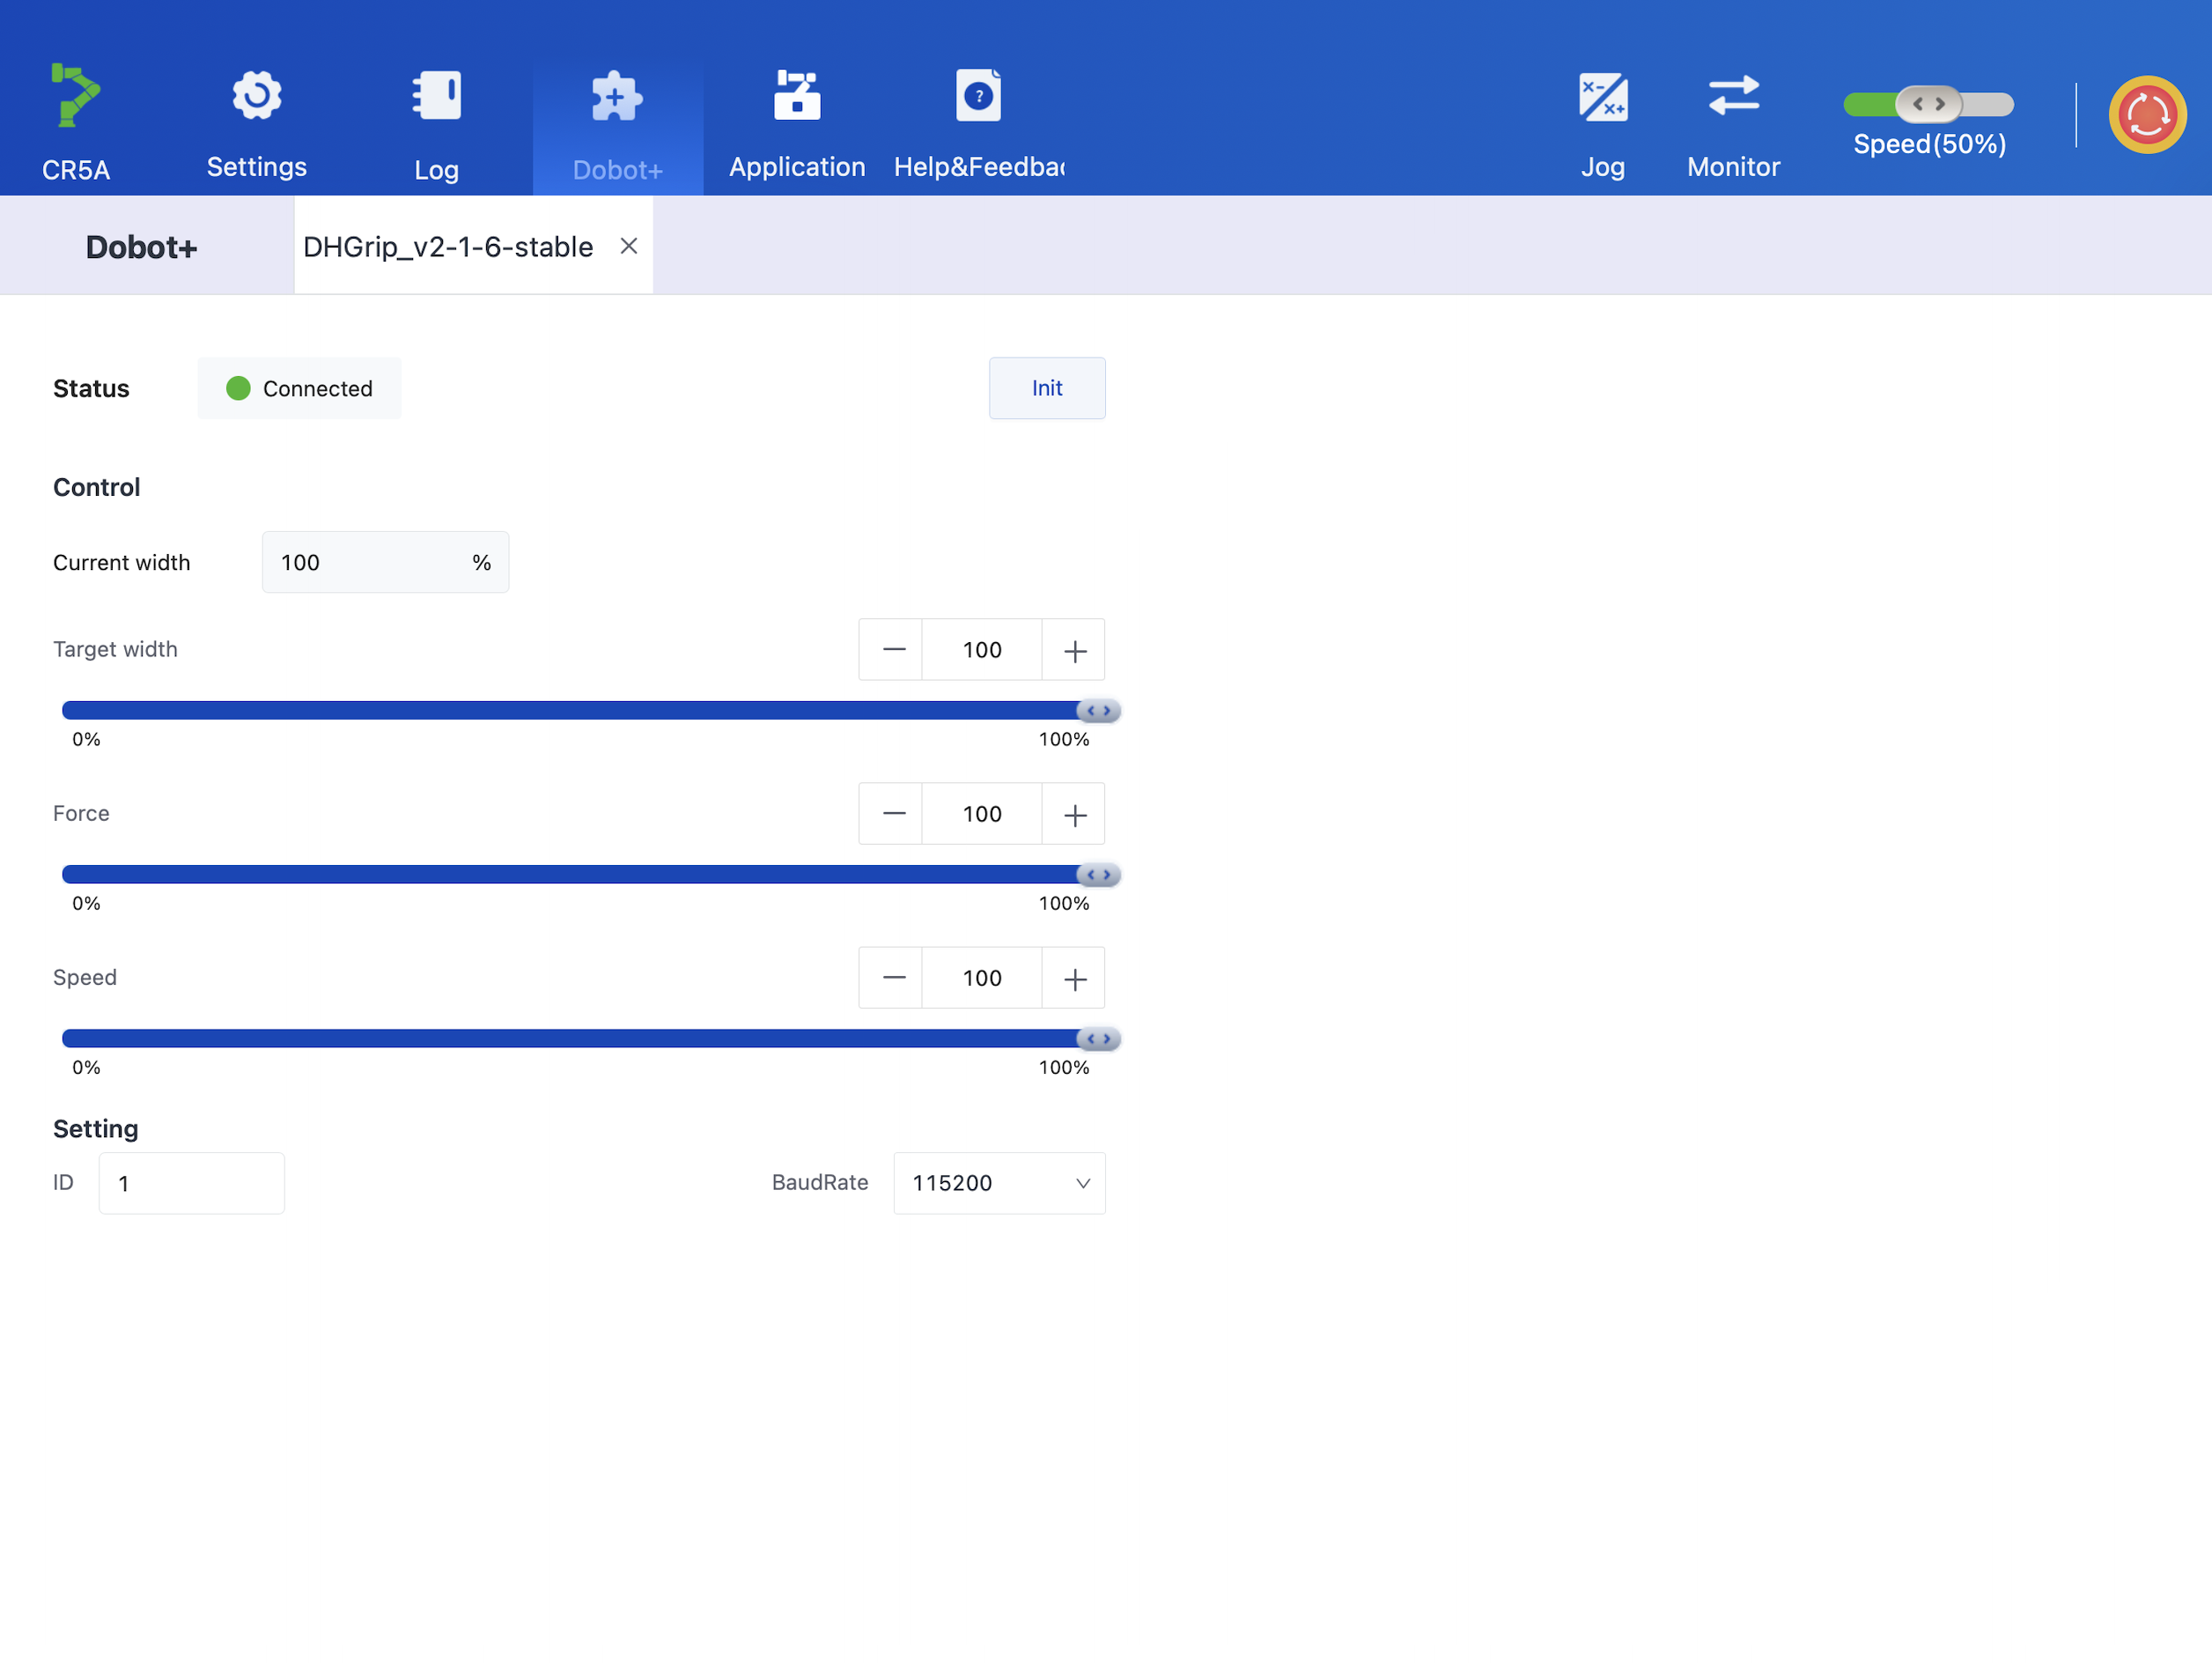
\includegraphics[width=0.9\textwidth]{12.png}
\end{figure}

\begin{figure}[H]
    \centering
    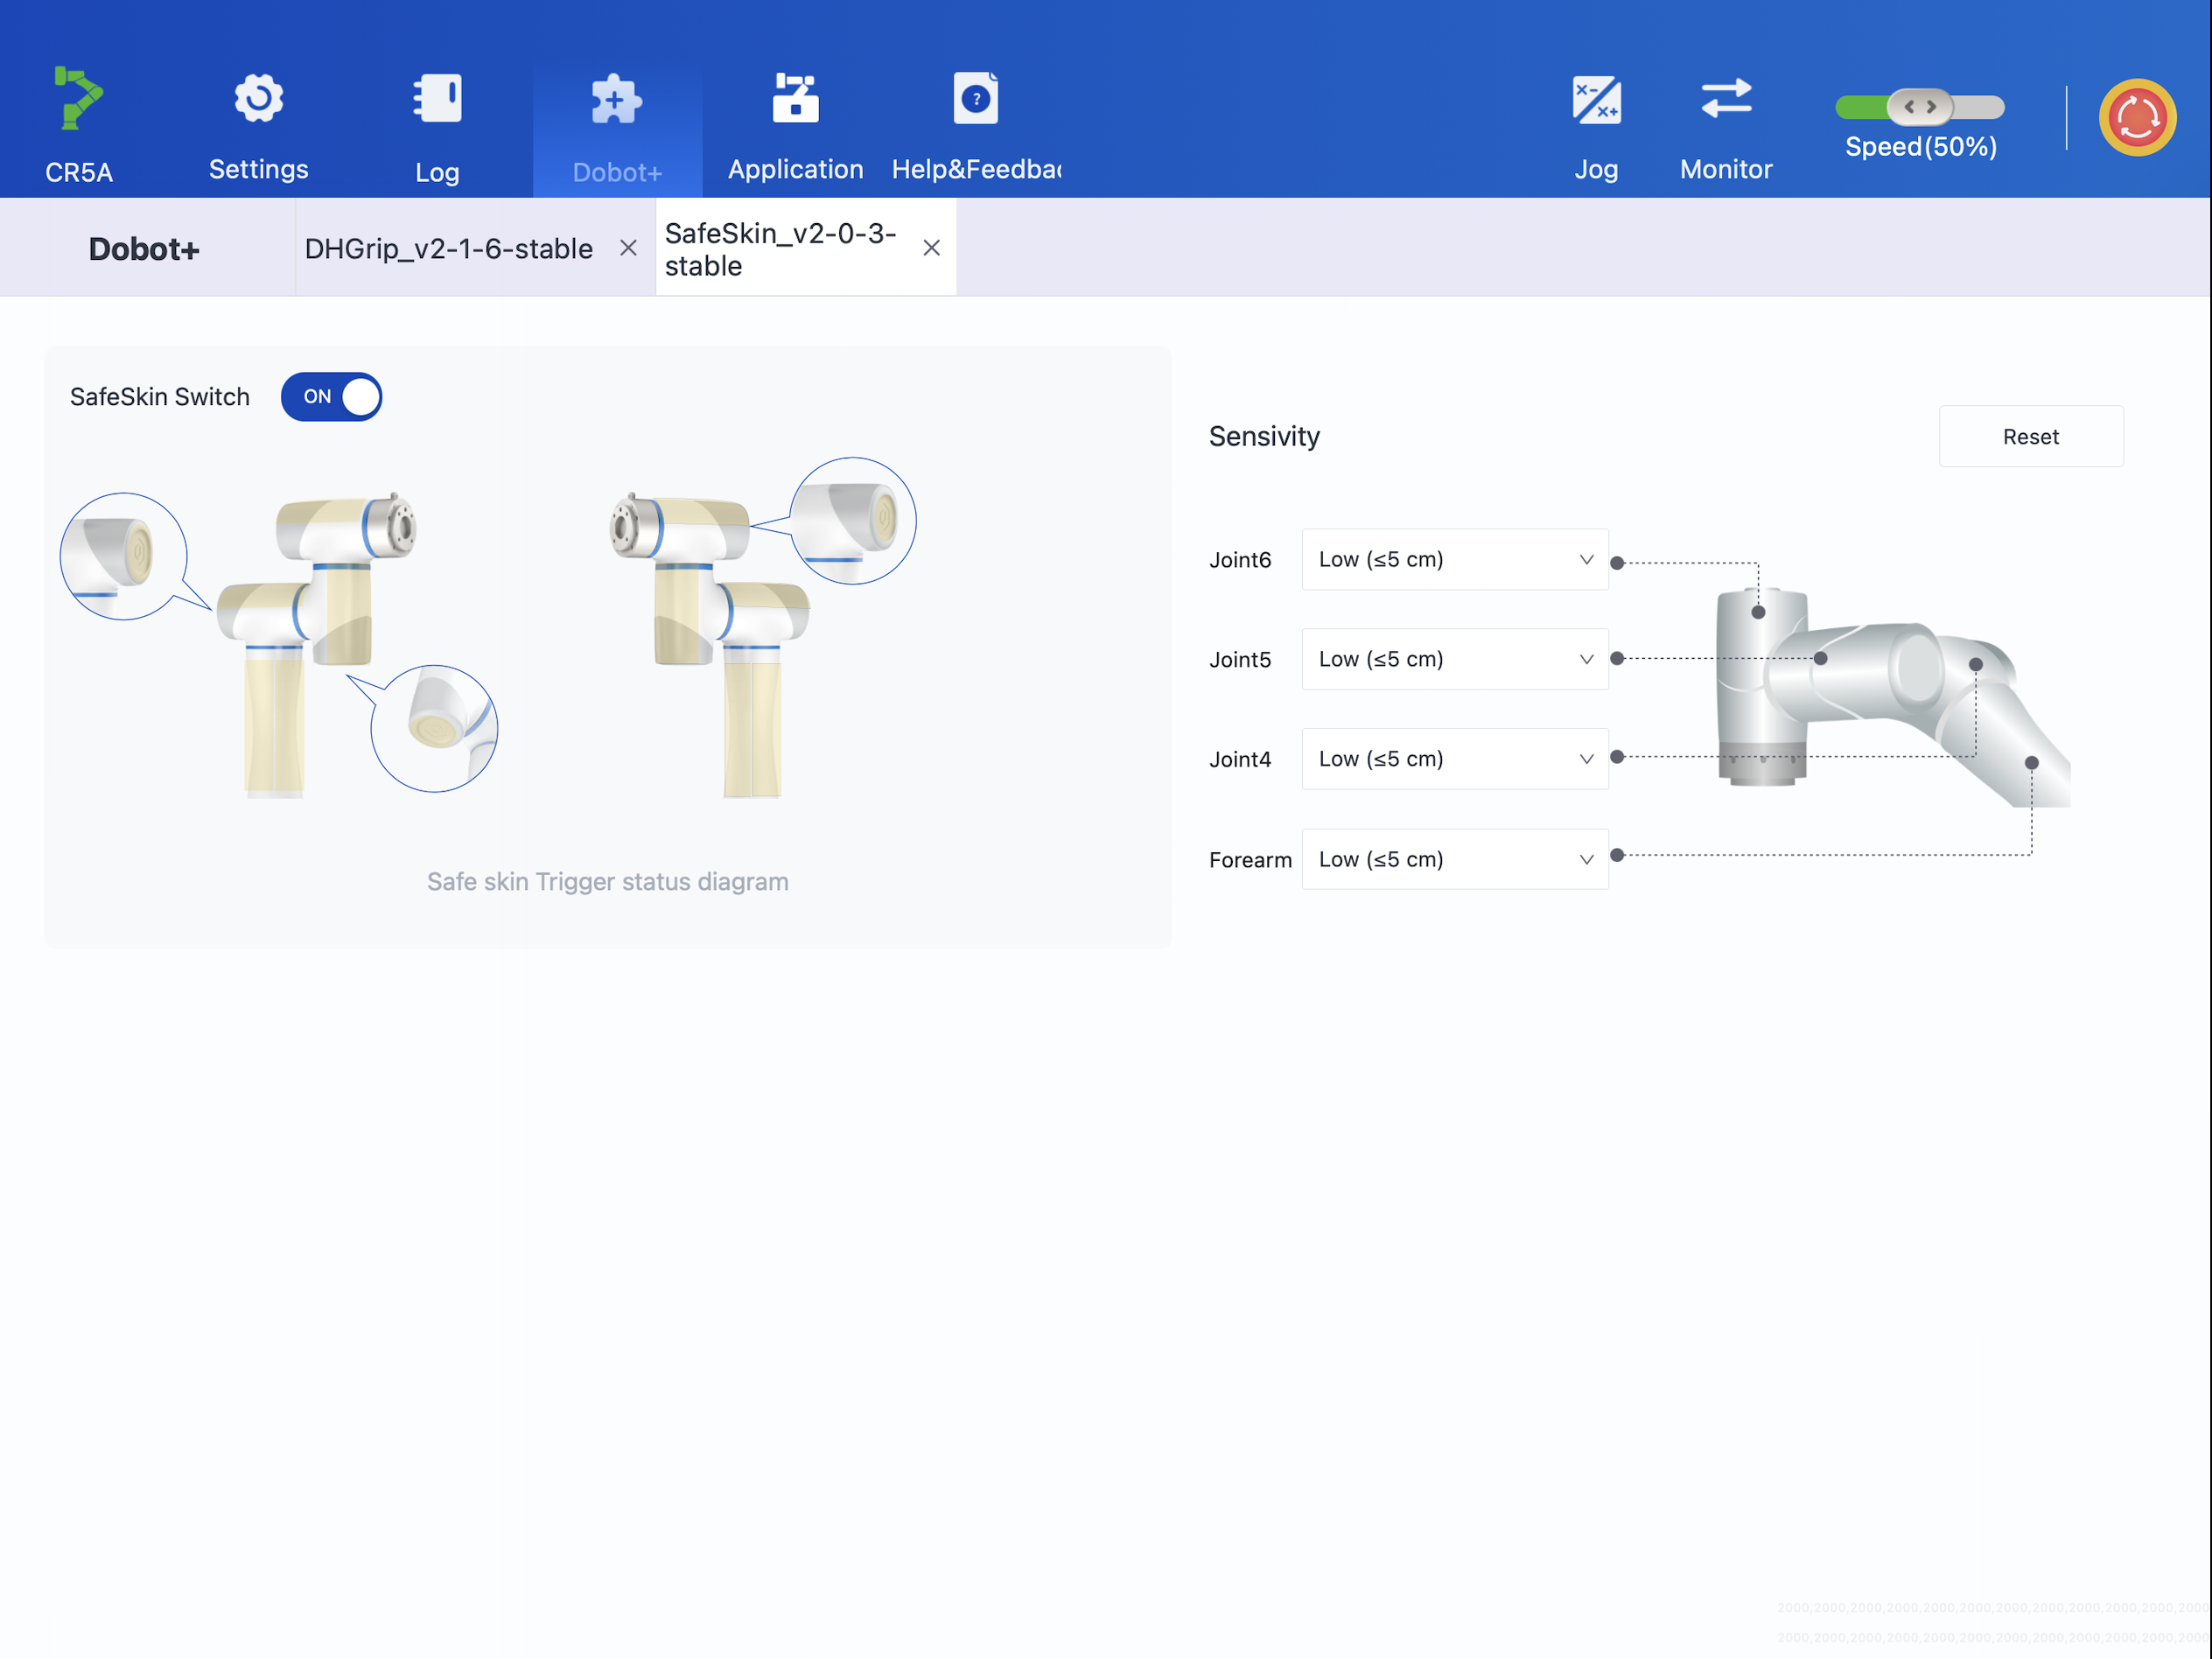
\includegraphics[width=0.9\textwidth]{13.png}
\end{figure}

\item Premendo ``Application'' potrai programmare il Dobot usando le funzioni del software. Hai la possibilità di usare la programmazione Blockly o la programmazione a Script. Entrambe sono valide e includono l'opzione ``Points'', che permette di registrare punti mentre sei in Drag Mode e utilizzarli nel tuo script.

\begin{figure}[H]
    \centering
    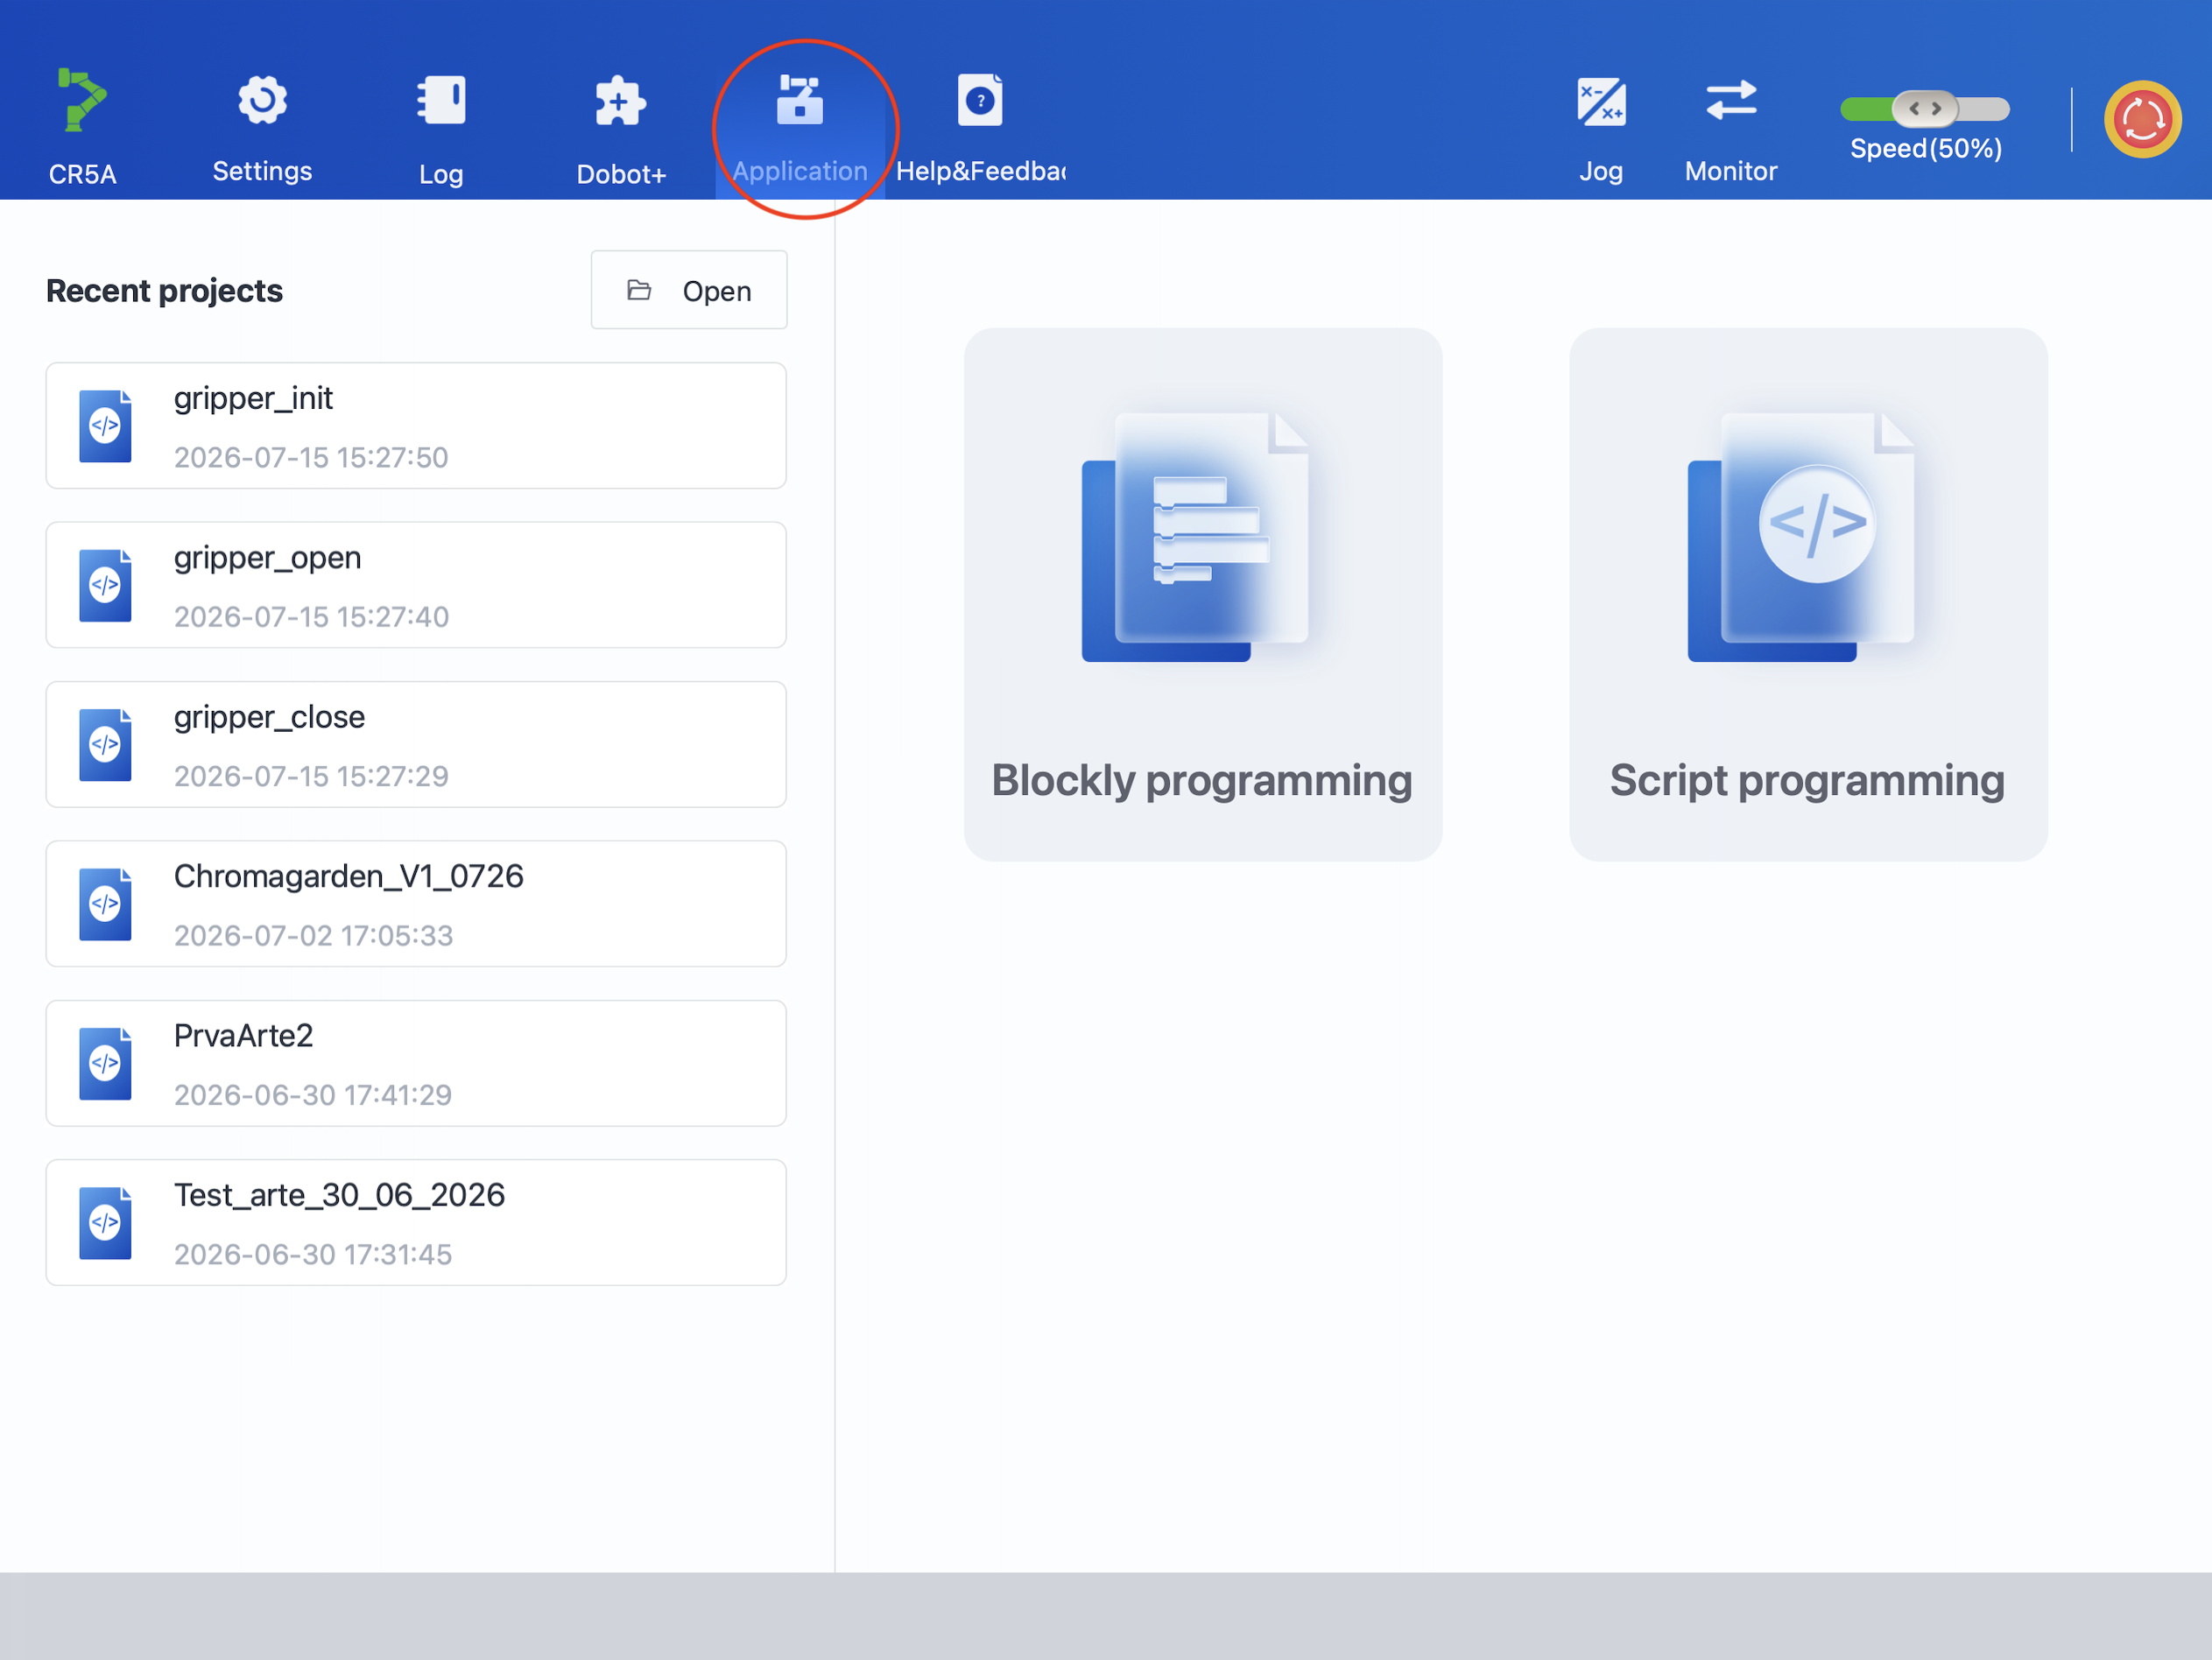
\includegraphics[width=0.9\textwidth]{14.png}
\end{figure}

\begin{figure}[H]
    \centering
    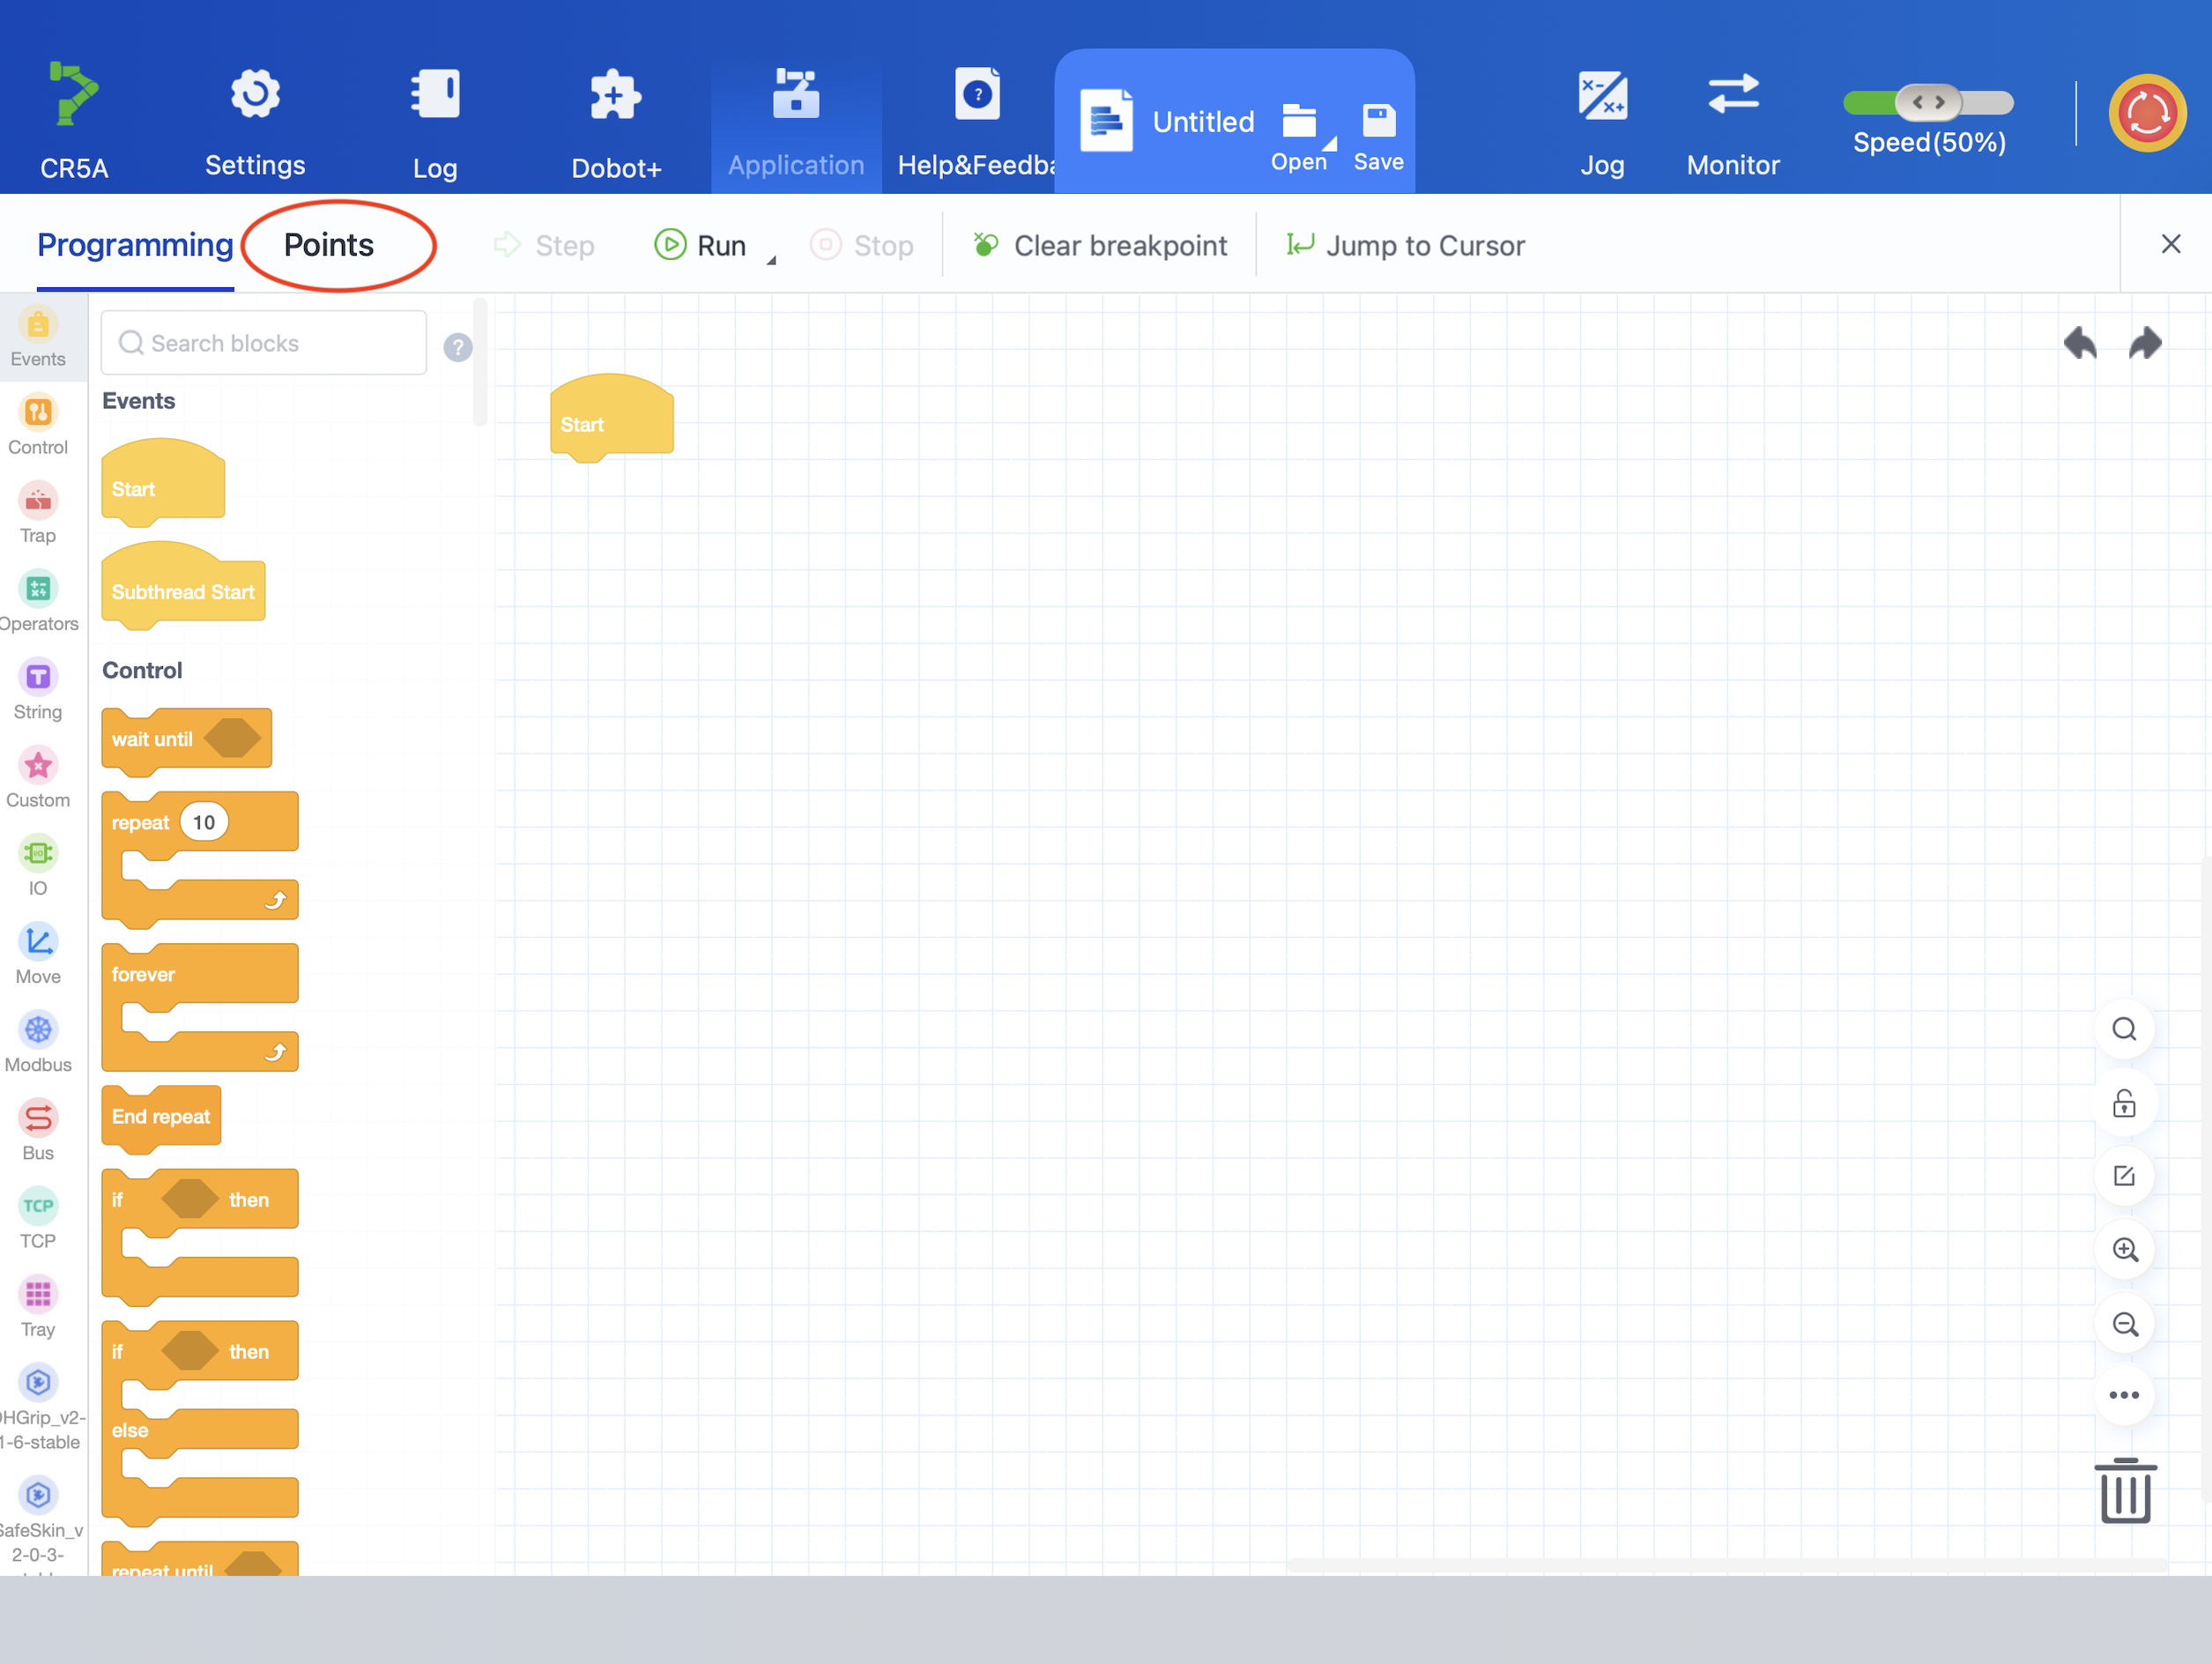
\includegraphics[width=0.9\textwidth]{15.png}
\end{figure}

\begin{figure}[H]
    \centering
    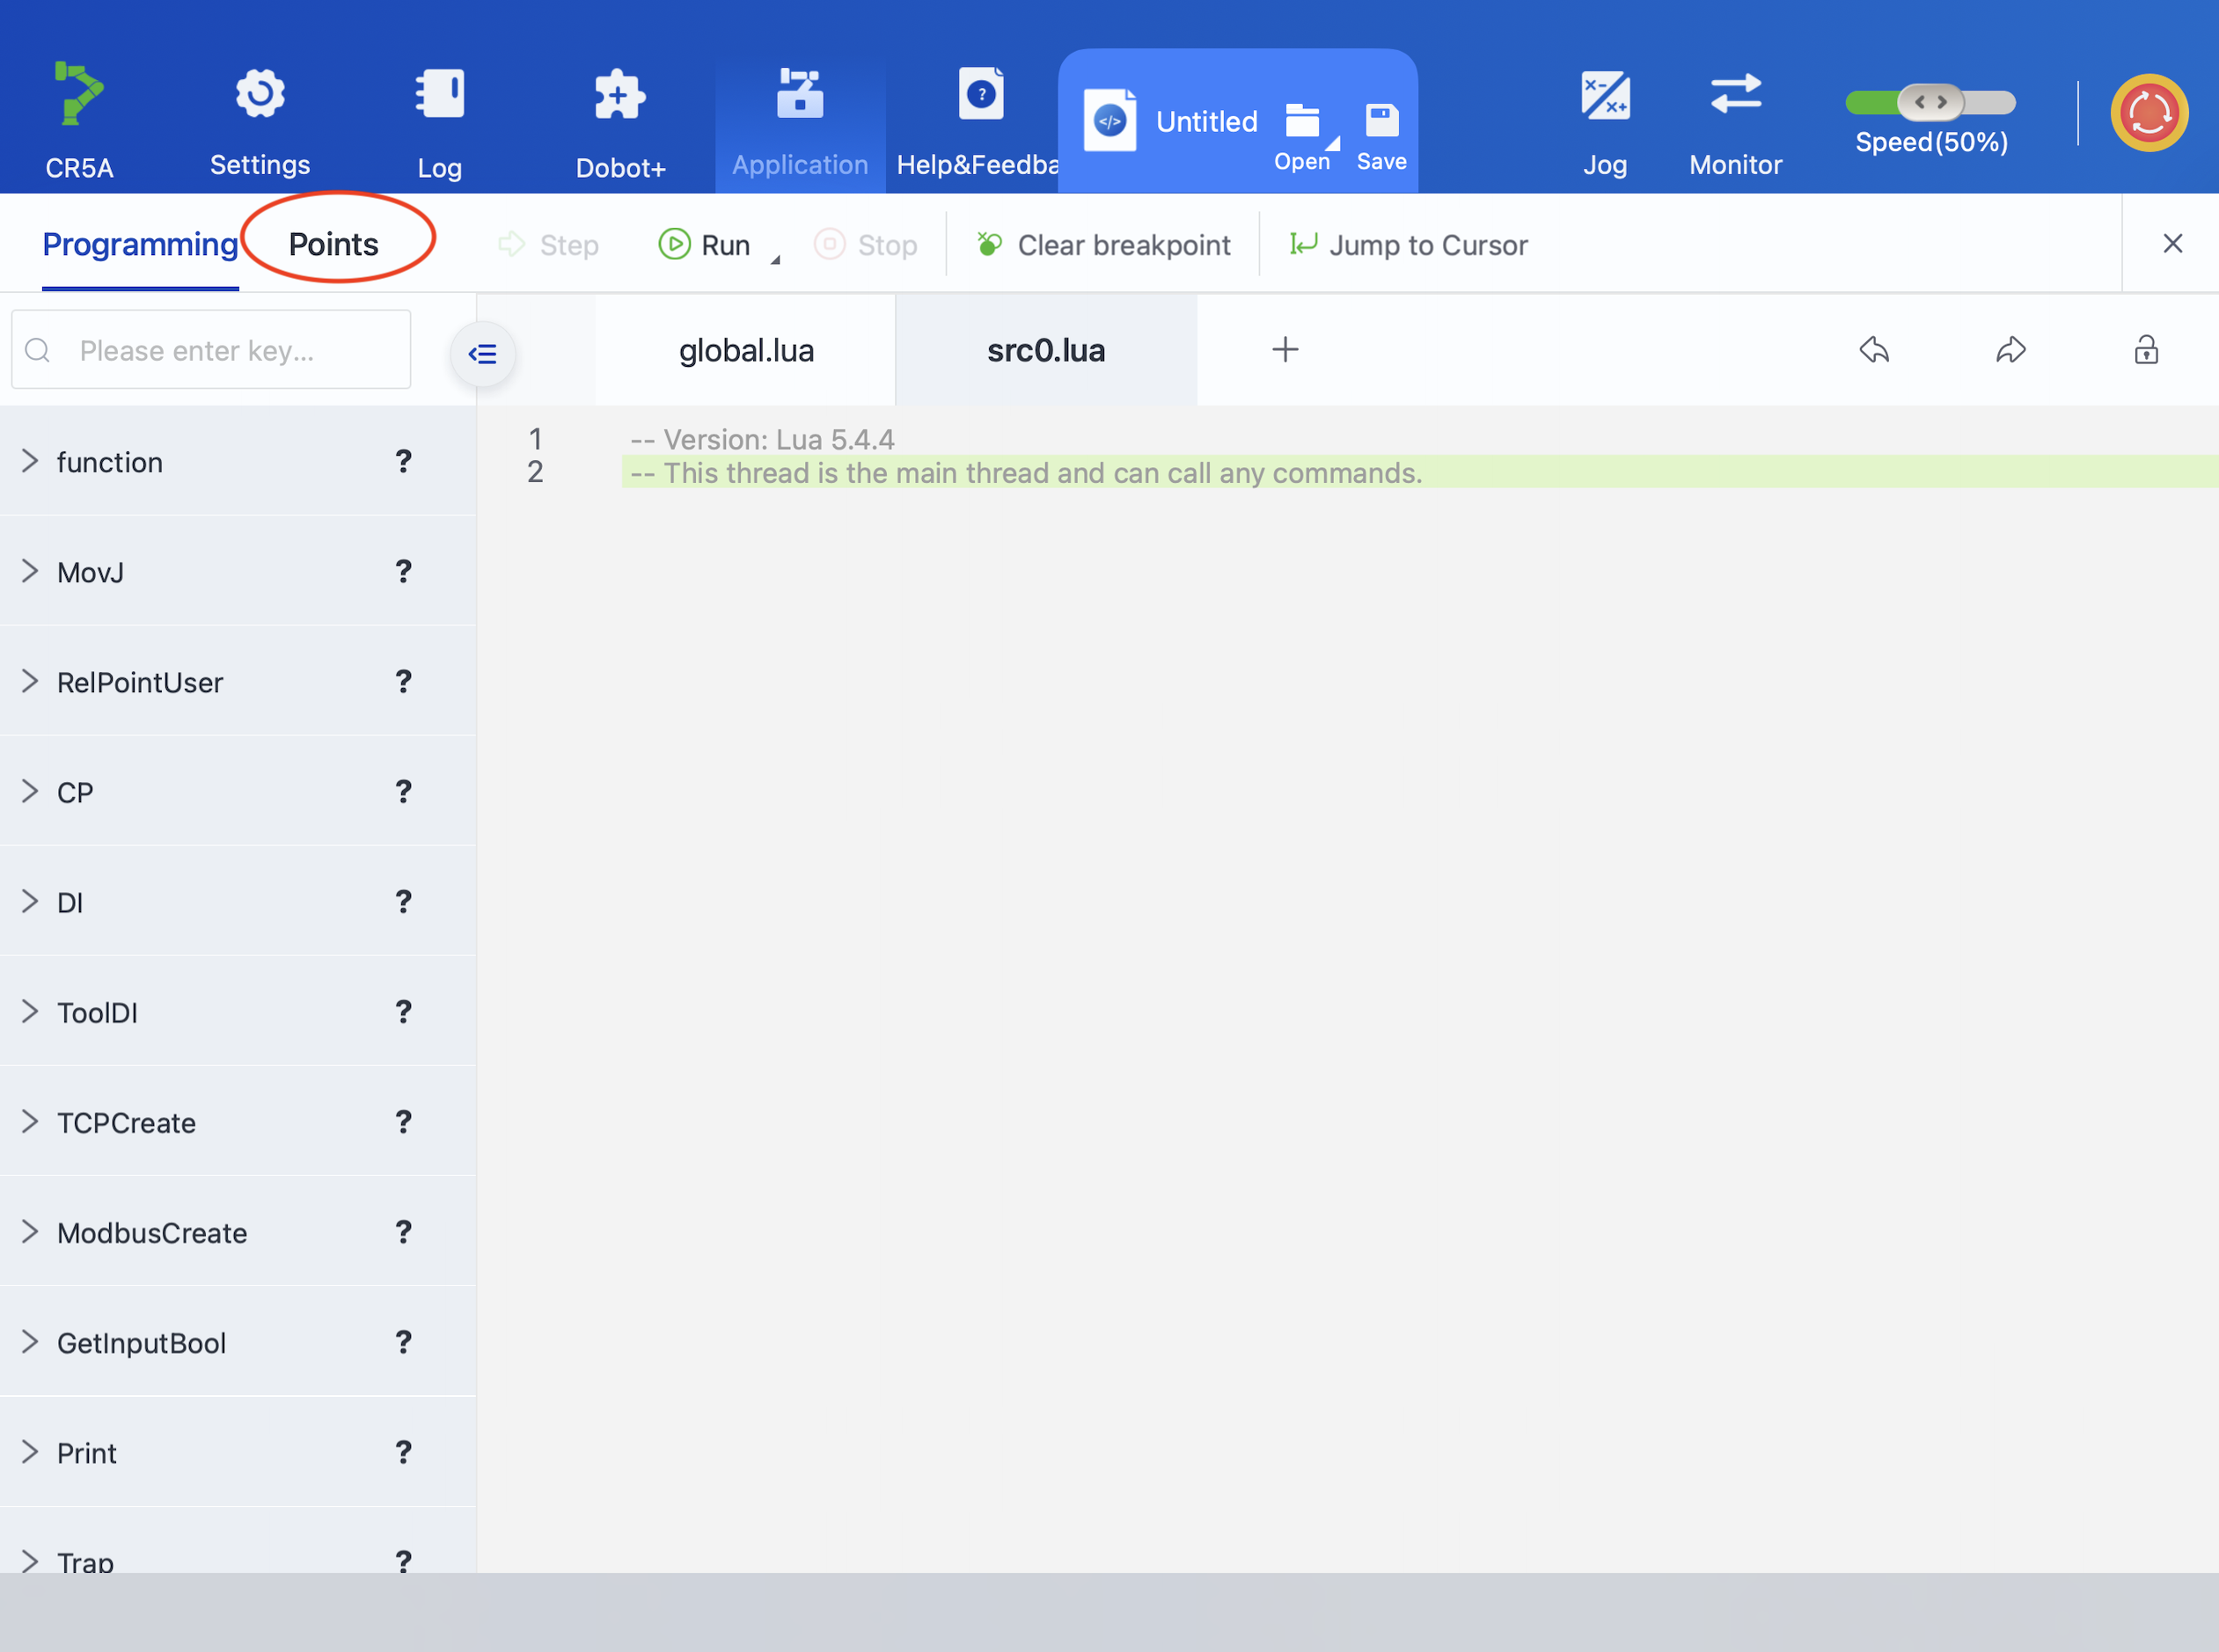
\includegraphics[width=0.9\textwidth]{16.png}
\end{figure}

\begin{figure}[H]
    \centering
    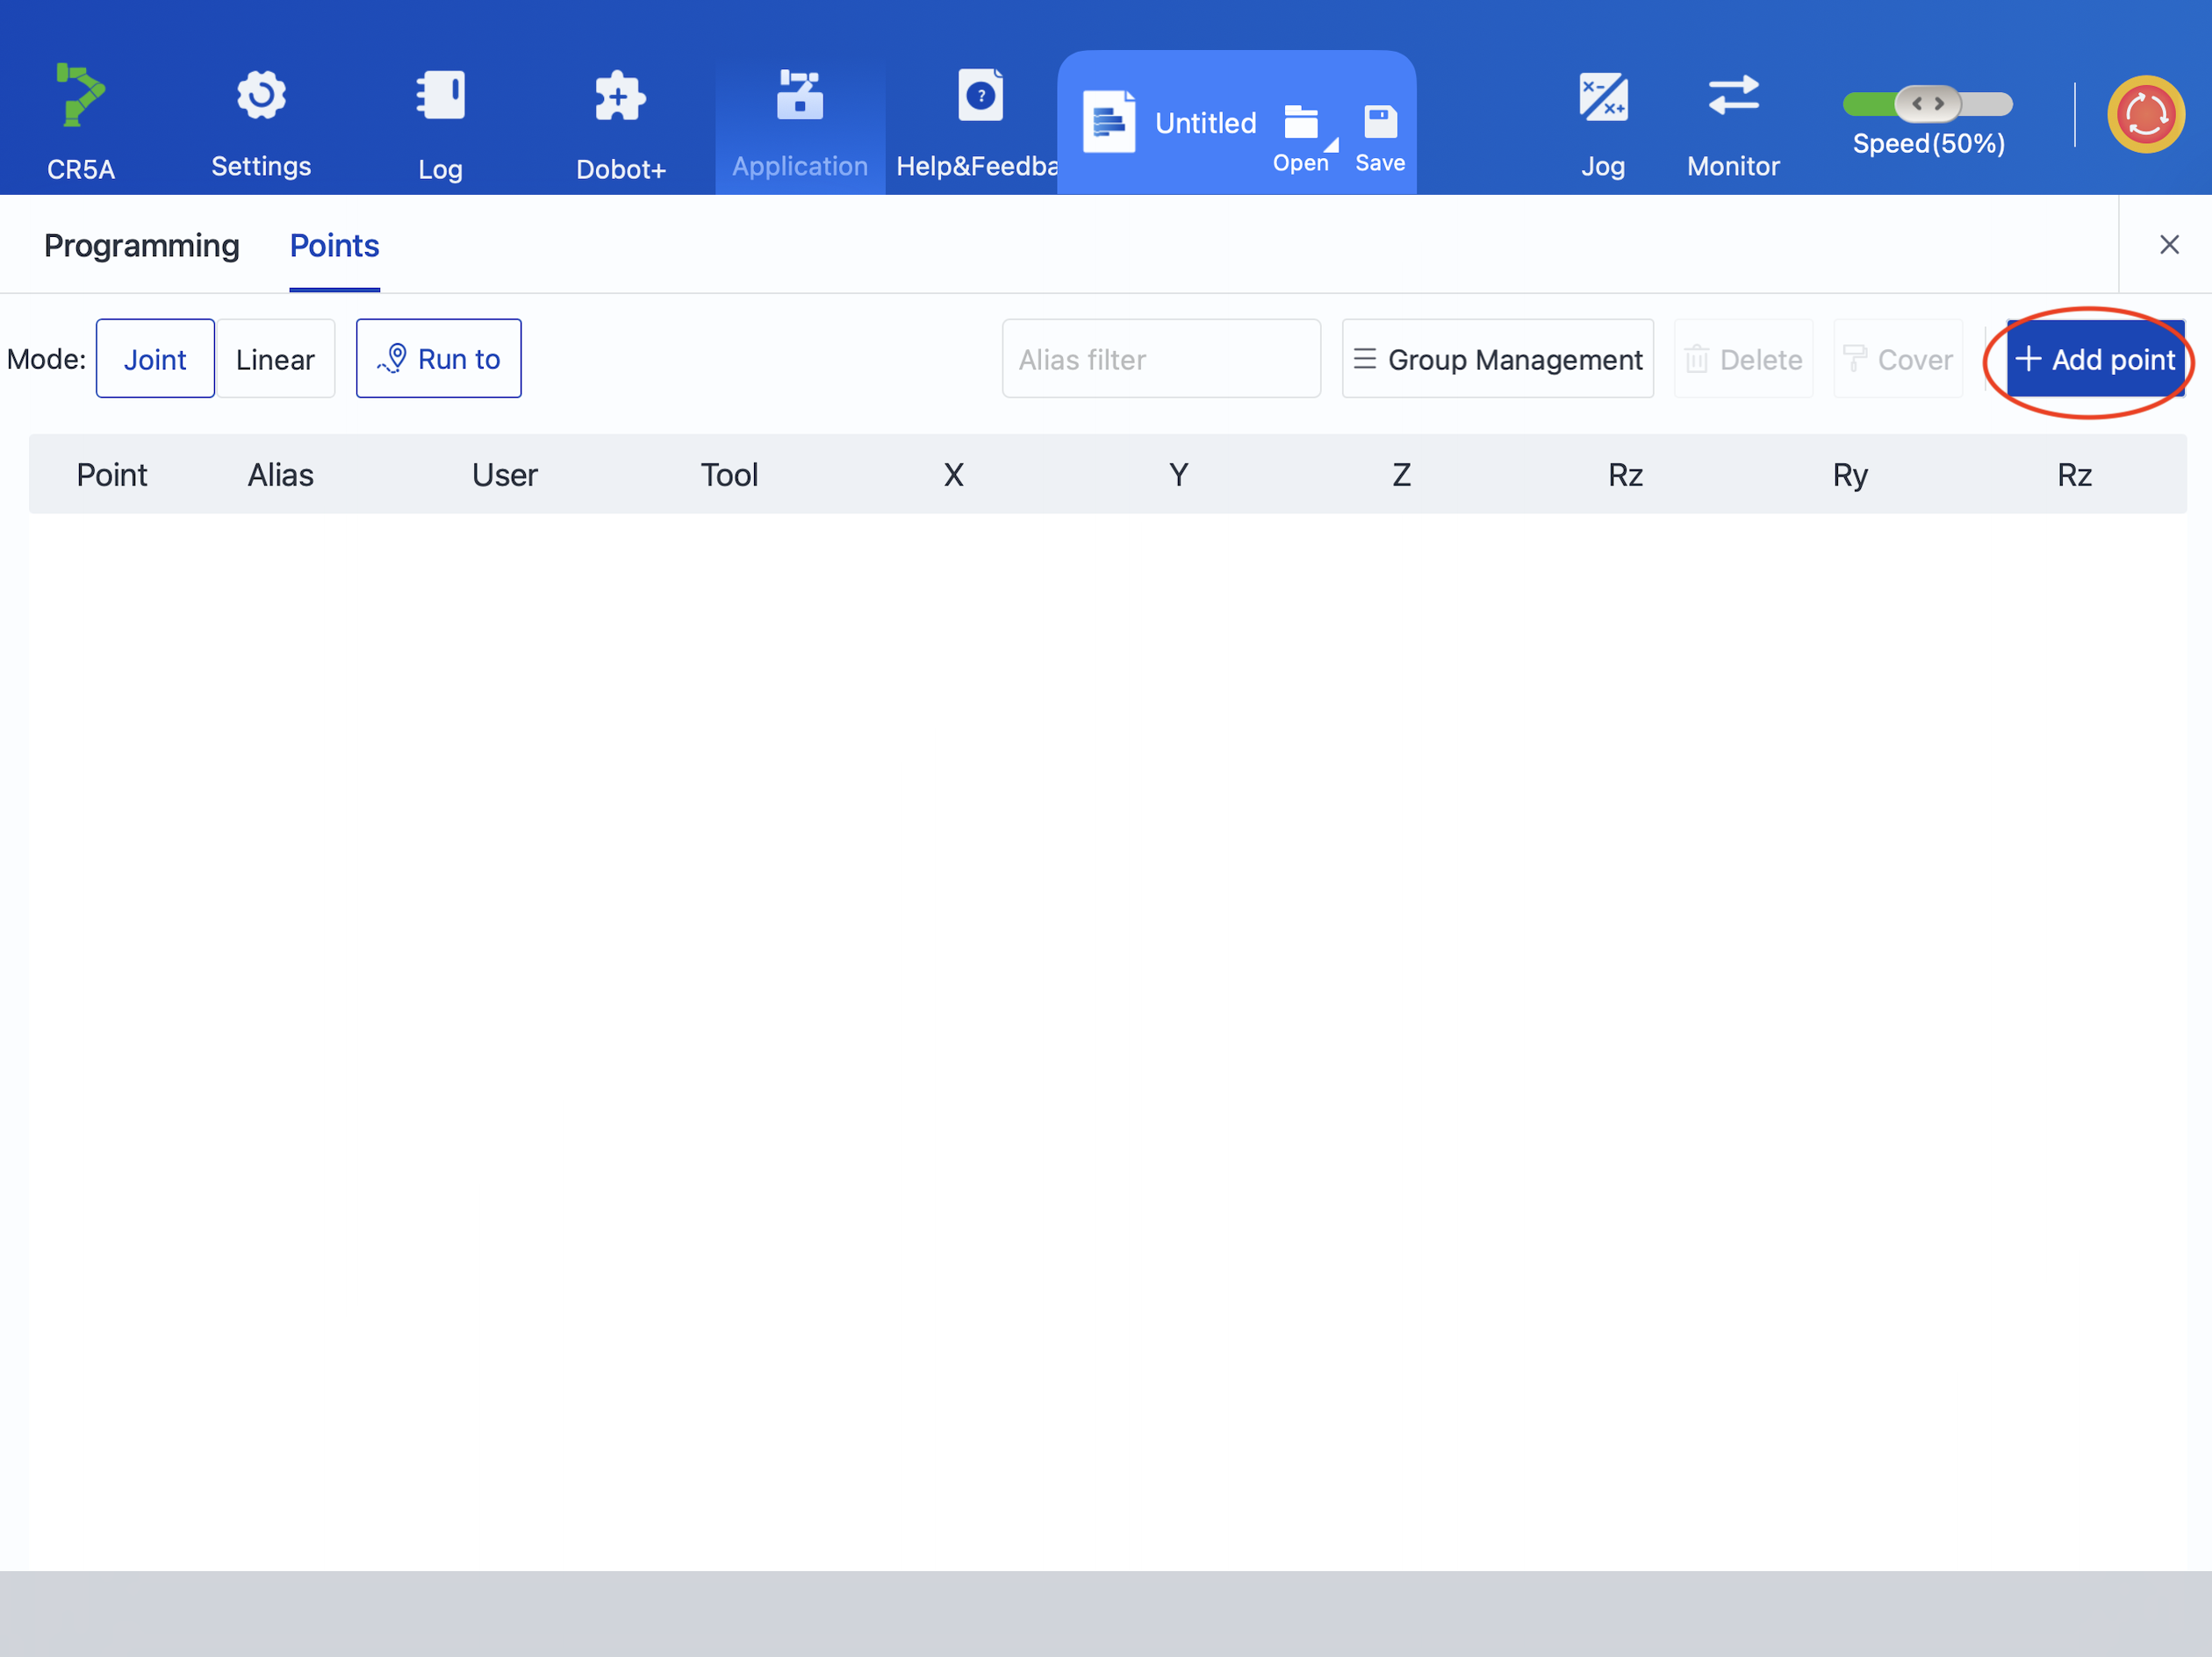
\includegraphics[width=0.9\textwidth]{17.png}
\end{figure}

\item Ogni volta che viene premuto il pulsante E-Stop, o si verifica un altro errore, puoi visualizzarlo ed eliminarlo dal pannello ``Log''.

Nota bene: ogni volta che il pulsante E-Stop viene premuto, dovrai disinnestarlo, cancellare l'allarme e poi tornare al pannello ``CR5A'' per riabilitare (Enable) il Dobot.

\begin{figure}[H]
    \centering
    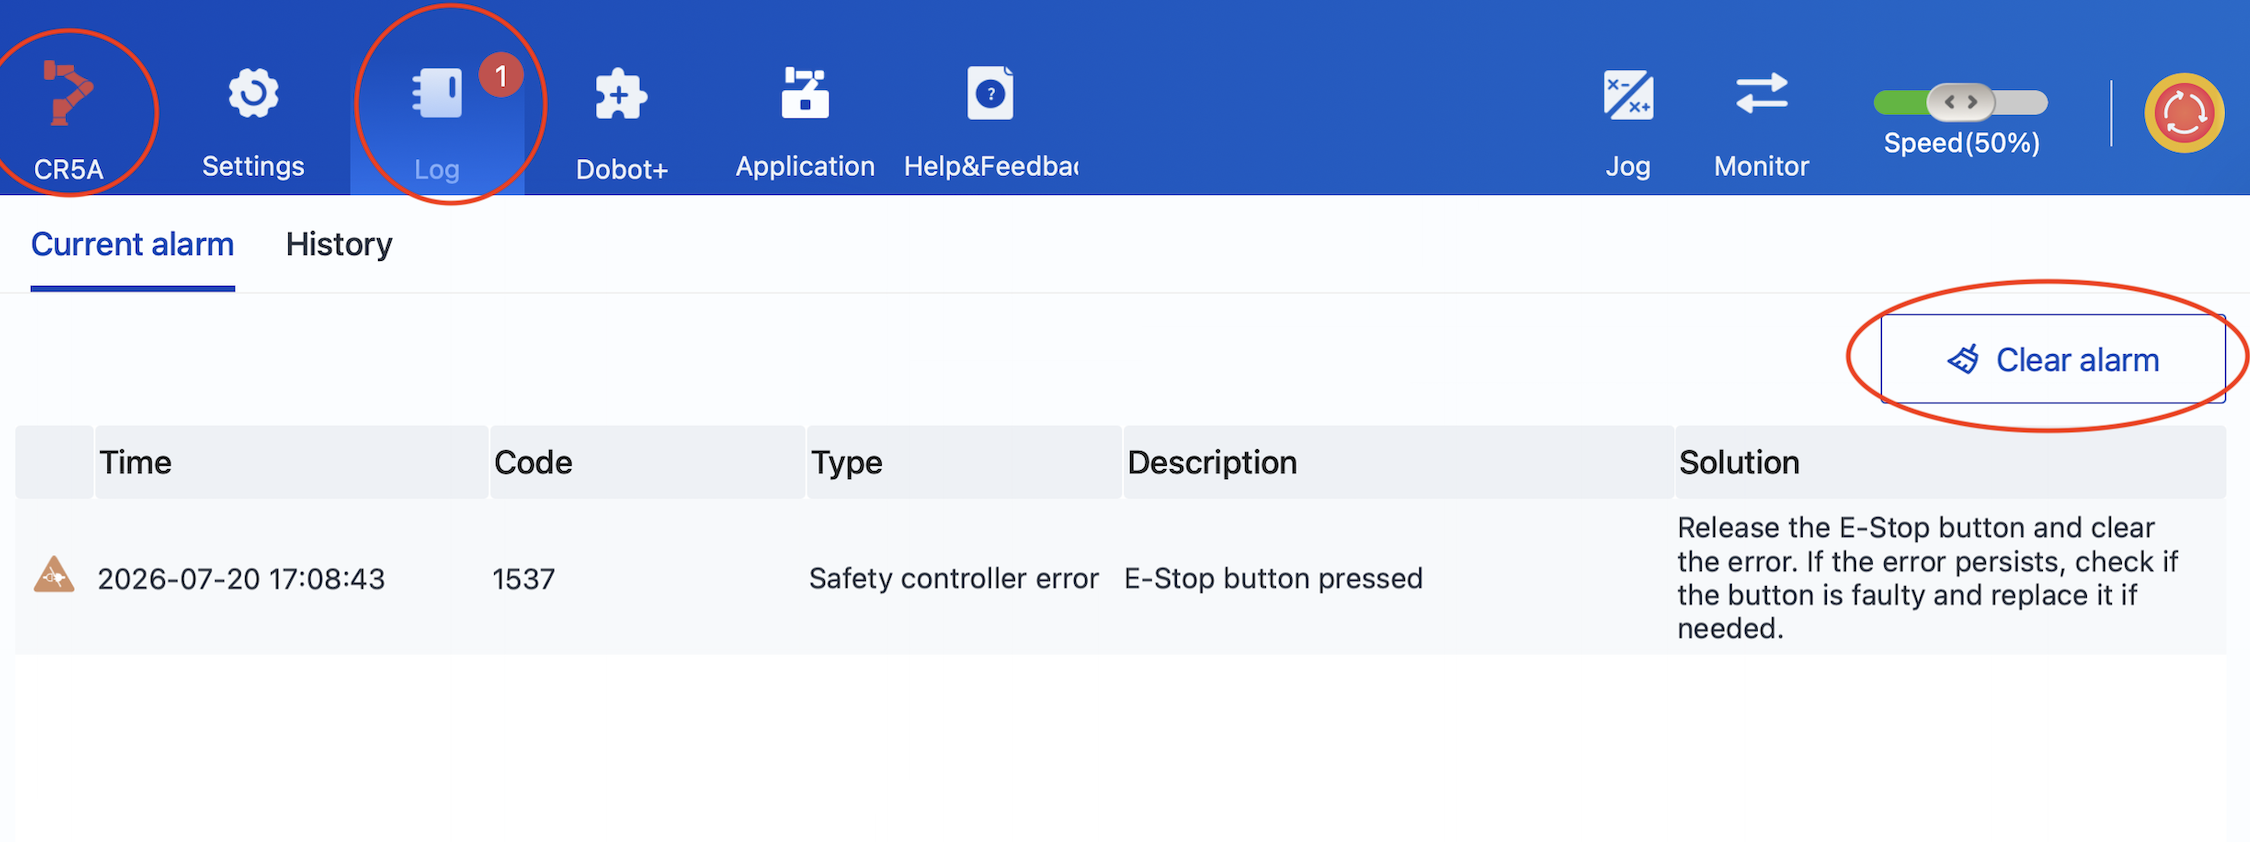
\includegraphics[width=0.9\textwidth]{18.png}
\end{figure}

\end{itemize}

% ============================================================
\section{Come programmare con script Python}
\label{sec:python-programming}
% ============================================================

Di seguito una breve spiegazione delle principali funzionalità e dei comandi che permettono di controllare il Dobot tramite script in modalità TCP.

La libreria che ho scelto di usare è quella ufficiale; è disponibile su GitHub all'indirizzo \url{https://github.com/Dobot-Arm/TCP-IP-Python-V4}, ma l'ho inserita anche nel repository a cui questo manuale è allegato.

Ecco un elenco di tutti i comandi che potrebbero essere utili:

\subsubsection*{Connessione / stato di alimentazione}
\begin{itemize}[leftmargin=1.2cm]
    \item \code{EnableRobot()} --- accende il braccio
    \item \code{DisableRobot()} --- lo spegne
    \item \code{ClearError()} --- azzera lo stato di allarme
\end{itemize}

\subsubsection*{Movimento}
\begin{itemize}[leftmargin=1.2cm]
    \item \code{MovJ()} --- movimento punto-punto nello spazio dei giunti
    \item \code{MovL()} --- movimento lineare (Cartesiano)
    \item \code{StartDrag()} --- entra in modalità drag/teach (guida manuale)
    \item \code{StopDrag()} --- esce dalla modalità drag
    \item \code{SpeedFactor()} --- imposta il rapporto di velocità globale
\end{itemize}

\subsubsection*{Stato / feedback}
\begin{itemize}[leftmargin=1.2cm]
    \item \code{RobotMode()} --- restituisce lo stato attuale del robot (abilitato, in esecuzione, errore, ecc.)
    \item \code{GetAngle()} --- legge gli angoli attuali dei giunti
    \item \code{GetPose()} --- legge la posizione Cartesiana attuale
\end{itemize}

\subsubsection*{Cinematica}
\begin{itemize}[leftmargin=1.2cm]
    \item \code{InverseKin()} --- converte un target Cartesiano in angoli dei giunti
\end{itemize}

\subsubsection*{Gripper / I/O dell'utensile}
\begin{itemize}[leftmargin=1.2cm]
    \item \code{SetToolPower()} --- attiva/disattiva l'alimentazione lato utensile (usato prima del controllo del gripper)
    \item \code{ToolDOInstant()} --- commuta istantaneamente un'uscita digitale dell'utensile, usato per aprire/chiudere il gripper
    \item \code{GetToolDO()} --- legge lo stato attuale dell'uscita digitale dell'utensile
\end{itemize}

\subsubsection*{Modbus (per i gripper che lo utilizzano, come il DH Robotics PGC-140-50)}
\begin{itemize}[leftmargin=1.2cm]
    \item \code{ModbusRTUCreate()} --- apre una connessione Modbus RTU verso il gripper (ID slave, baud rate, parità, bit di dati, bit di stop)
    \item \code{ModbusClose()} --- chiude quella connessione Modbus
\end{itemize}

Per controllare un gripper DH puoi usare il protocollo Modbus (sconsigliato, poiché richiederebbe di avere il gripper collegato al computer principale del Dobot con un cavo non sempre incluso) oppure il protocollo Remote Control, che fa eseguire al codice Python script già scritti in DobotStudio Pro. Quest'ultima è l'opzione migliore e richiede solo una configurazione iniziale che può risultare macchinosa, ma è molto più semplice da usare in seguito.

\subsection*{Controllo remoto per il gripper DH}

\textbf{Configurazione:}

\begin{enumerate}[leftmargin=1.2cm]
    \item Disattiva la modalità TCP.
    \item Connetti il Dobot a DobotStudio Pro.
    \item Scarica il plug-in del gripper DH dall'elenco fornito nel software.
    \item Nella sezione di programmazione del software, aggiungi i 3 script principali (sono inclusi nella cartella ``Examples'', in una cartella che specifica che si tratta degli script Lua collegati all'Example 11, che muove il gripper).
    \item Attiva la modalità TCP. Ora potrai attivare questi 3 script secondo necessità (vedi la cartella ``Examples'' per la struttura del codice). L'unico accorgimento è che devi tenere il software DobotStudio Pro sempre aperto in background, altrimenti non funzionerà correttamente.
\end{enumerate}

Ho aggiunto un file di esempio nel repository GitHub per ciascuno di questi, nella cartella ``Examples''. Per eseguirli correttamente, scarica la cartella ``Examples'', decomprimila ed esegui il file che ti interessa. La libreria Dobot è già inclusa in questa cartella per un uso più semplice. Con altre librerie potresti semplicemente scaricarle sul tuo PC senza doverle referenziare ogni volta, ma questa libreria non ha un file \code{setup.py}, quindi qui non è possibile farlo.

\begin{longtable}{@{}p{5cm}p{9.5cm}@{}}
\toprule
\textbf{File di esempio} & \textbf{Cosa fa} \\
\midrule
\endhead
\code{00_hello_world.py} & Si connette, abilita il robot, e muove J1 avanti e indietro da 0\textdegree{} a +/- 30\textdegree{} per mostrare lo schema base connessione $\rightarrow$ abilitazione $\rightarrow$ movimento $\rightarrow$ disabilitazione. \\ \midrule
\code{01_connect_and_status.py} & Si connette, azzera gli errori, abilita il robot, e legge il suo stato attuale tramite \code{RobotMode()}. \\ \midrule
\code{02_joint_motion.py} & Mostra il movimento nello spazio dei giunti con \code{MovJ()}, spostando J1 a 30\textdegree{} e leggendo gli angoli dei giunti prima/dopo con \code{GetAngle()}. \\ \midrule
\code{03_linear_motion_and_pose.py} & Mostra il movimento lineare con \code{MovL()}, sollevando l'utensile di 50mm sull'asse Z usando coordinate Cartesiane lette tramite \code{GetPose()}. \\ \midrule
\code{04_drag_mode.py} & Mette il robot in modalità drag a guida manuale (\code{StartDrag()}/\code{StopDrag()}) così puoi muoverlo manualmente e leggere la posizione risultante. \\ \midrule
\code{05_inverse_kinematics.py} & Usa \code{InverseKin()} per calcolare quali angoli dei giunti richiederebbe una posizione target X/Y/Z, senza muoversi realmente lì. \\ \midrule
\code{06_drag_record_and_replay.py} & Ti permette di trascinare il robot in più posizioni, registra gli angoli dei giunti di ciascuna alla pressione di Invio, poi riproduce l'intera sequenza con \code{MovJ()}. \\ \midrule
\code{07_interactive_joint_jog.py} & Un ciclo interattivo che chiede quale giunto muovere e a quale angolo, poi muove solo quel giunto. \\ \midrule
\code{08_record_cartesian_points.py} & Stessa idea del file 06, ma registra/riproduce posizioni Cartesiane X/Y/Z (\code{GetPose()}/\code{MovL()}) invece di angoli dei giunti. \\ \midrule
\code{09_closest_reachable_position.py} & Prova a raggiungere un target X/Y/Z indicato dall'utente e, se irraggiungibile, arretra passo dopo passo (Z, poi Y, poi X) finché non trova un punto raggiungibile. \\ \midrule
\code{10_speed_comparison_test.py} & Ripete lo stesso movimento di J1 (0\textdegree$\rightarrow$180\textdegree) con cinque diverse impostazioni di \code{SpeedFactor()} così puoi confrontare come la velocità influenza il movimento. \\ \midrule
\code{11_gripper_init_open_close.py} & Attiva gli script Lua di init/chiusura/apertura del gripper tramite un socket grezzo e riabilita il robot (\code{ClearError()} + \code{EnableRobot()}) dopo ciascuno di essi. \\
\bottomrule
\end{longtable}

\subsection{Informazioni aggiuntive}
\label{sec:additional-info}

\begin{itemize}[leftmargin=1.2cm]

\item Mentre usi il software DobotStudio Pro, puoi attivare la Drag Mode premendo il pulsante fisico su J6 del Dobot per 4 secondi, finché il LED non inizia a lampeggiare viola, e disattivarla premendolo una volta. Se SafeSkin è attivo, cosa consigliata sempre, potrebbe darti un errore mentre provi a raggiungere il pulsante. Puoi evitarlo abbassando temporaneamente la precisione di SafeSkin nelle impostazioni, ricordandoti però di riportarla alla normalità quando hai finito con la Drag Mode.

\item Quando usi la cinematica inversa (Inverse Kinematics), sia in modalità TCP che TP, potresti spesso ottenere un errore che indica che la posizione non è raggiungibile, anche se saresti stato in grado di posizionare il robot lì con la Drag Mode. Questo è dovuto ai calcoli matematici alla base di questa funzione, che sono molto precisi e potrebbero riuscire a raggiungere un punto molto vicino a quello selezionato, di alcuni millimetri di distanza (cosa che in Drag Mode non noti), ma non quel punto specifico. Potresti risolvere questo problema permettendo al Dobot di raggiungere il punto disponibile più vicino a quello selezionato, oppure aggiungendo un'altra libreria di cinematica inversa.

\end{itemize}

\end{document}